% =============================================================================
%  M\'etaheuristiques pour le Probl\`eme d'Ordonnancement de Flow Shop de Permutation
%  \'Etude Comparative: NEH vs SMA vs GWO vs GA
%  Auteur: ZARQI Ezzoubair — Juin 2026
% =============================================================================

\documentclass[12pt,a4paper,oneside]{report}

% ==========================================
% PACKAGES
% ==========================================
\usepackage{mathpazo}
\usepackage{geometry}
\usepackage{graphicx}
\usepackage{xcolor}
\usepackage{hyperref}
\usepackage{fancyhdr}
\usepackage{titlesec}
\usepackage{float}
\usepackage{microtype}
\usepackage{setspace}
\usepackage{listings}
\usepackage[most]{tcolorbox}
\usepackage{fontawesome5}
\usepackage{booktabs}
\usepackage{array}
\usepackage{colortbl}
\usepackage{mdframed}
\usepackage{enumitem}
\usepackage{tikz}
\usetikzlibrary{shapes, arrows.meta, positioning, calc, decorations.pathreplacing}
\usepackage{pgfplots}
\pgfplotsset{compat=1.18}
\usepackage{multicol}
\usepackage{caption}
\usepackage{subcaption}
\usepackage{amsmath}
\usepackage{amssymb}
\usepackage{multirow}
\usepackage{algorithm}
\usepackage{algpseudocode}
\usepackage[french]{babel}

% ==========================================
% PALETTE DE COULEURS
% ==========================================
\definecolor{PrimaryBlue}{RGB}{15, 52, 96}
\definecolor{AccentBlue}{RGB}{52, 120, 246}
\definecolor{LightBlue}{RGB}{235, 243, 255}
\definecolor{DarkGray}{RGB}{45, 45, 55}
\definecolor{MidGray}{RGB}{110, 110, 125}
\definecolor{LightGray}{RGB}{245, 246, 250}
\definecolor{BorderGray}{RGB}{220, 222, 230}
\definecolor{OliveGreen}{RGB}{46, 125, 50}

\definecolor{InfoBlue}{RGB}{0, 122, 204}
\definecolor{InfoBlueBg}{RGB}{232, 244, 255}
\definecolor{InfoBlueBorder}{RGB}{144, 202, 249}
\definecolor{SuccessGreen}{RGB}{22, 128, 72}
\definecolor{SuccessGreenBg}{RGB}{232, 250, 240}
\definecolor{SuccessGreenBorder}{RGB}{134, 210, 172}
\definecolor{WarningAmber}{RGB}{160, 100, 0}
\definecolor{WarningAmberBg}{RGB}{255, 248, 230}
\definecolor{WarningAmberBorder}{RGB}{245, 200, 120}
\definecolor{DangerRed}{RGB}{185, 28, 28}
\definecolor{DangerRedBg}{RGB}{255, 235, 235}
\definecolor{DangerRedBorder}{RGB}{240, 150, 150}
\definecolor{TipPurple}{RGB}{90, 40, 180}
\definecolor{TipPurpleBg}{RGB}{245, 238, 255}
\definecolor{TipPurpleBorder}{RGB}{195, 165, 245}

\definecolor{CodeBg}{RGB}{250, 251, 253}
\definecolor{CodeComment}{RGB}{100, 160, 100}
\definecolor{CodeKeyword}{RGB}{0, 80, 200}
\definecolor{CodeString}{RGB}{180, 30, 30}
\definecolor{CodeNumber}{RGB}{140, 60, 180}
\definecolor{CodeLineNo}{RGB}{170, 172, 185}
\definecolor{CodeBorder}{RGB}{200, 210, 230}

% ── Algorithm colors ────────────────────────────────────────────────────────
\definecolor{smaColor}{HTML}{2196F3}
\definecolor{gwoColor}{HTML}{9C27B0}
\definecolor{gaColor}{HTML}{FF5722}
\definecolor{nehColor}{HTML}{4CAF50}
\definecolor{randColor}{HTML}{FF9800}

% ==========================================
% CONFIGURATION DU DOCUMENT
% ==========================================
\geometry{top=2.8cm, bottom=2.8cm, left=2.8cm, right=2.5cm, marginparwidth=0cm}
\setstretch{1.15}

\hypersetup{
    colorlinks=true,
    linkcolor=AccentBlue,
    filecolor=AccentBlue,
    urlcolor=AccentBlue,
    pdftitle={M\'etaheuristiques pour le Probl\`eme d'Ordonnancement de Flow Shop de Permutation},
    pdfauthor={ZARQI Ezzoubair},
    bookmarksnumbered=true,
    pdfpagemode=UseOutlines
}

% ==========================================
% TITRES ET SECTIONS
% ==========================================
\titleformat{\chapter}[display]
  {\color{PrimaryBlue}\normalfont\Huge\bfseries}
  {\color{AccentBlue}\small\bfseries\sffamily CHAPITRE \thechapter}
  {4pt}
  {
    \rule{\textwidth}{1.5pt}\vspace{6pt}
    \begin{minipage}{\textwidth}
      \raggedright\color{PrimaryBlue}
  }
  [
    \end{minipage}
    \vspace{4pt}\rule{\textwidth}{0.4pt}
  ]
\titlespacing*{\chapter}{0pt}{0pt}{28pt}

\titleformat{\section}
  {\color{PrimaryBlue}\normalfont\Large\bfseries}
  {\color{AccentBlue}\thesection}{1em}{}
  [\color{BorderGray}\titlerule]
\titlespacing*{\section}{0pt}{20pt}{10pt}

\titleformat{\subsection}
  {\color{PrimaryBlue}\normalfont\large\bfseries}
  {\color{AccentBlue}\thesubsection}{1em}{}
\titlespacing*{\subsection}{0pt}{14pt}{6pt}

% ==========================================
% EN-TETES ET PIEDS DE PAGE
% ==========================================
\pagestyle{fancy}
\fancyhf{}
\fancyhead[L]{%
  \textcolor{MidGray}{\small\sffamily PFSP --- \'Etude Comparative de M\'ehtaheuristiques}%
}
\fancyhead[R]{%
  \textcolor{MidGray}{\small\sffamily\thepage}%
}
\fancyfoot[L]{\textcolor{MidGray}{\scriptsize\sffamily Auteur: ZARQI Ezzoubair}}
\fancyfoot[C]{\textcolor{MidGray}{\scriptsize\sffamily Juin 2026}}
\fancyfoot[R]{\textcolor{MidGray}{\scriptsize\sffamily Universite Abdelmalek Essaadi --- FST Tanger}}
\renewcommand{\headrulewidth}{0.4pt}
\renewcommand{\headrule}{\hbox to\headwidth{\color{BorderGray}\leaders\hrule height\headrulewidth\hfill}}
\renewcommand{\footrulewidth}{0.4pt}
\renewcommand{\footrule}{\hbox to\headwidth{\color{BorderGray}\leaders\hrule height\footrulewidth\hfill}}

% ==========================================
% STYLE CODE SOURCE
% ==========================================
\lstdefinestyle{PythonCode}{
    language=Python,
    backgroundcolor=\color{CodeBg},
    basicstyle=\ttfamily\footnotesize,
    keywordstyle=\color{CodeKeyword}\bfseries,
    stringstyle=\color{CodeString},
    commentstyle=\color{CodeComment}\itshape,
    numberstyle=\tiny\color{CodeLineNo},
    numbers=left,
    numbersep=12pt,
    stepnumber=1,
    tabsize=4,
    showspaces=false,
    showstringspaces=false,
    breaklines=true,
    breakatwhitespace=true,
    frame=none,
    xleftmargin=20pt,
    xrightmargin=8pt,
}

\lstset{
  basicstyle=\ttfamily\small,
  breaklines=true,
  frame=single,
  numbers=left,
  numberstyle=\tiny,
  backgroundcolor=\color{gray!5},
  keywordstyle=\color{blue!80},
  commentstyle=\color{green!50!black},
  showstringspaces=false,
}

% ==========================================
% CARTES SEMANTIQUES
% ==========================================
\newtcolorbox{cardinfo}[1][]{
    enhanced, breakable,
    colback=InfoBlueBg, colframe=InfoBlueBorder,
    arc=5pt, boxrule=0.8pt,
    left=38pt, right=8pt, top=6pt, bottom=6pt,
    overlay={
        \begin{tcbclipinterior}
            \fill[InfoBlue] (frame.north west) rectangle ([xshift=28pt]frame.south west);
            \node[text=white, font=\Large\bfseries] at ([xshift=14pt, yshift=0pt]frame.west) {\faInfoCircle};
        \end{tcbclipinterior}
    },
    detach title, before upper={\textbf{\textcolor{InfoBlue}{\sffamily Information}}\par\smallskip},
    #1
}

\newtcolorbox{cardsuccess}[1][]{
    enhanced, breakable,
    colback=SuccessGreenBg, colframe=SuccessGreenBorder,
    arc=5pt, boxrule=0.8pt,
    left=38pt, right=8pt, top=6pt, bottom=6pt,
    overlay={
        \begin{tcbclipinterior}
            \fill[SuccessGreen] (frame.north west) rectangle ([xshift=28pt]frame.south west);
            \node[text=white, font=\Large\bfseries] at ([xshift=14pt]frame.west) {\faCheckCircle};
        \end{tcbclipinterior}
    },
    detach title, before upper={\textbf{\textcolor{SuccessGreen}{\sffamily Succ\`es}}\par\smallskip},
    #1
}

\newtcolorbox{cardwarning}[1][]{
    enhanced, breakable,
    colback=WarningAmberBg, colframe=WarningAmberBorder,
    arc=5pt, boxrule=0.8pt,
    left=38pt, right=8pt, top=6pt, bottom=6pt,
    overlay={
        \begin{tcbclipinterior}
            \fill[WarningAmber] (frame.north west) rectangle ([xshift=28pt]frame.south west);
            \node[text=white, font=\Large\bfseries] at ([xshift=14pt]frame.west) {\faExclamationTriangle};
        \end{tcbclipinterior}
    },
    detach title, before upper={\textbf{\textcolor{WarningAmber}{\sffamily Attention}}\par\smallskip},
    #1
}

\newtcolorbox{cardtip}[1][]{
    enhanced, breakable,
    colback=TipPurpleBg, colframe=TipPurpleBorder,
    arc=5pt, boxrule=0.8pt,
    left=38pt, right=8pt, top=6pt, bottom=6pt,
    overlay={
        \begin{tcbclipinterior}
            \fill[TipPurple] (frame.north west) rectangle ([xshift=28pt]frame.south west);
            \node[text=white, font=\Large\bfseries] at ([xshift=14pt]frame.west) {\faLightbulb};
        \end{tcbclipinterior}
    },
    detach title, before upper={\textbf{\textcolor{TipPurple}{\sffamily Astuce}}\par\smallskip},
    #1
}

% ==========================================
% LEGENDES
% ==========================================
\captionsetup{
    font=small,
    labelfont={bf, color=PrimaryBlue},
    labelsep=period,
    skip=6pt
}

% ==========================================
% LISTES PERSONNALISEES
% ==========================================
\setlist[itemize,1]{
    label=\textcolor{AccentBlue}{\small\faChevronRight},
    leftmargin=1.5em,
    itemsep=3pt
}
\setlist[enumerate,1]{
    label=\textcolor{AccentBlue}{\bfseries\arabic*.},
    leftmargin=1.8em,
    itemsep=3pt
}

% =============================================================================
\begin{document}

% ==========================================
% PAGE DE GARDE
% ==========================================
\begin{titlepage}
    \newcommand{\HRule}{\textcolor{PrimaryBlue}{\rule{\linewidth}{0.6pt}}}

    \thispagestyle{empty}
    \begin{center}
        \vspace*{0.4cm}

        % ---- Logos ----
        \noindent
        \begin{minipage}[c]{0.48\textwidth}
            \raggedright
            \includegraphics[height=2.0cm,keepaspectratio]{logo-uae-1024x297.png}
        \end{minipage}%
        \begin{minipage}[c]{0.48\textwidth}
            \raggedleft
            \includegraphics[height=2.3cm,keepaspectratio]{fst-1024x383.png}
        \end{minipage}

        \vspace{0.6cm}
        \textcolor{BorderGray}{\rule{\linewidth}{0.4pt}}
        \vspace{0.3cm}

        % ---- Etablissement ----
        {\large\textsc{\color{PrimaryBlue} Universite Abdelmalek Essaadi}}\\[0.25cm]
        {\normalsize\color{MidGray} Faculte des Sciences et Techniques --- Tanger}\\[0.15cm]
        {\normalsize\textsc{\color{PrimaryBlue} Departement d'Informatique}}

        \vspace{2.6cm}

        % ---- Titre ----
        \HRule\\[0.45cm]
        {\huge\bfseries\color{PrimaryBlue} Metaheuristics for the\\[0.3cm] Permutation Flow Shop\\[0.3cm] Scheduling Problem}\\[0.3cm]
        {\large\color{MidGray} A Comparative Study: NEH -- SMA -- GWO -- GA}\\[0.35cm]
        \HRule

        \vspace{2.8cm}

        % ---- Auteurs ----
        \noindent
        \begin{minipage}[t]{0.48\textwidth}
            \begin{flushleft}\large
                \textcolor{MidGray}{\small\bfseries\sffamily Author:}\\[0.3cm]
                \textsc{ZARQI Ezzoubair}
            \end{flushleft}
        \end{minipage}%
        \begin{minipage}[t]{0.48\textwidth}
            \begin{flushright}\large
                \textcolor{MidGray}{\small\bfseries\sffamily Supervisor:}\\[0.3cm]
                Pr. \textsc{Nom et Prenom}
            \end{flushright}
        \end{minipage}

        \vfill

        % ---- Pied de page garde ----
        \textcolor{BorderGray}{\rule{\linewidth}{0.4pt}}\\[0.4cm]
        {\normalsize\textbf{Projet:} M\'etaheuristiques pour le PFSP --- NEH, SMA, GWO, GA
        \\
         \textbf{Fili\`ere:} Master --- Intelligence Artificielle \& Data Science
         \quad\textcolor{BorderGray}{|}\quad
         \textbf{Ann\'ee:} 2025 -- 2026}
        \vspace*{0.6cm}

    \end{center}
\end{titlepage}

% ── Table of Contents ───────────────────────────────────────────────────────
\tableofcontents
\clearpage

% =============================================================================
%  CHAPTER 1 — Introduction
% =============================================================================
\chapter{Introduction}

\section{Probl\`eme d'Ordonnancement de Flow Shop de Permutation (PFSP)}

Le probl\`eme d'ordonnancement de flow shop de permutation (PFSP) est l'un des probl\`emes d'optimisation combinatoire les plus \'etudi\'es dans la litt\'erature d'ordonnancement. Le probl\`eme est d\'efini comme suit:

\begin{itemize}[itemsep=4pt]
    \item $n$ \textbf{t\^aches} doivent \^etre trait\'ees sur $m$ \textbf{machines}.
    \item Chaque t\^ache $j$ n\'ecessite un temps de traitement $p_{j,k}$ sur la machine $k$.
    \item Toutes les t\^aches visitent les machines dans le \textbf{m\^eme ordre} (flow shop).
    \item La s\'equence des t\^aches est \textbf{identique sur chaque machine} (contrainte de permutation).
    \item Chaque machine peut traiter au plus une t\^ache \`a la fois, et chaque t\^ache peut \^etre trait\'ee sur au plus une machine \`a la fois.
    \item La pr\'emption n'est pas autoris\'ee.
\end{itemize}

L'objectif est de \textbf{minimiser le makespan} $C_{\max}$, d\'efini comme le temps d'ach\`evement de la derni\`ere t\^ache sur la derni\`ere machine. Pour une permutation donn\'ee $\pi = (\pi_1, \pi_2, \dots, \pi_n)$, le makespan est calcul\'e r\'ecursivement:

\begin{equation}\label{eq:makespan}
\begin{aligned}
C_{\pi_1, 1} &= p_{\pi_1, 1} \\[2pt]
C_{\pi_1, k} &= C_{\pi_1, k-1} + p_{\pi_1, k}, \quad k = 2,\dots,m \\[2pt]
C_{\pi_i, 1} &= C_{\pi_{i-1}, 1} + p_{\pi_i, 1}, \quad i = 2,\dots,n \\[2pt]
C_{\pi_i, k} &= \max\bigl(C_{\pi_{i-1}, k},\; C_{\pi_i, k-1}\bigr) + p_{\pi_i, k}, \quad i=2,\dots,n;\; k=2,\dots,m
\end{aligned}
\end{equation}

Finalement, $C_{\max}(\pi) = C_{\pi_n, m}$.

\subsection{Complexit\'e Calculatoire}

Le PFSP avec $n$ t\^aches et $m$ machines poss\`ede un espace de recherche de $n!$ permutations possibles, rendant les m\'ethodes exactes (branch-and-bound, programmation dynamique, programmation lin\'eaire en nombres entiers) irr\'ealisables pour des instances au-del\`a d'environ $n=15$ t\^aches. Cette croissance exponentielle motive l'utilisation d'approches heuristiques et m\'etaheuristiques.

\begin{table}[H]
\centering
\begin{tabular}{c|c}
\toprule
$n$ (t\^aches) & $n!$ (taille de l'espace de solutions) \\
\midrule
10  & $3.63 \times 10^{6}$ \\
20  & $2.43 \times 10^{18}$ \\
50  & $3.04 \times 10^{64}$ \\
100 & $9.33 \times 10^{157}$ \\
\bottomrule
\end{tabular}
\caption{Croissance de l'espace de recherche du PFSP avec le nombre de t\^aches $n$.}
\label{tab:search-space}
\end{table}

\section{Approche: M\'etaheuristiques Continues avec Codage LOV}

Ce projet applique quatre algorithmes au PFSP:

\begin{enumerate}[itemsep=4pt]
    \item \textbf{NEH} — l'heuristique constructive de Nawaz--Enscore--Ham (r\'ef\'erence d\'eterministe, Nawaz et al., 1983).
    \item \textbf{SMA} — l'Algorithme du Physarum Polycephalum (Li et al., 2020).
    \item \textbf{GWO} — l'Optimiseur \`a Loups Gris (Mirjalili et al., 2014).
    \item \textbf{GA} — un Algorithme G\'en\'etique avec croisement BLX-$\alpha$ (Eshelman \& Schaffer, 1993).
\end{enumerate}

\'Etant donn\'e que SMA, GWO et GA sont des optimiseurs intrins\`equement \textbf{continus} (ils font \'evoluer des vecteurs dans $\mathbb{R}^n$), et que le PFSP est un probl\`eme de \textbf{permutation discret}, un codage \textbf{Largest Order Value (LOV)} est utilis\'e: chaque vecteur continu $X \in [0, 1]^n$ est d\'ecod\'e en une permutation en triant les indices selon leurs valeurs, i.e., $\pi = \operatorname{argsort}(X)$.

\section{Structure du Projet}

L'impl\'ementation est organis\'ee comme un package Python avec les modules suivants:

\begin{itemize}
    \item \texttt{pfsp.py} — D\'efinition du probl\`eme PFSP: calcul du makespan, heuristique NEH, op\'erateurs de recherche locale et g\'en\'eration d'instances (style Taillard).
    \item \texttt{sma.py} — Algorithme du Physarum Polycephalum (optimiseur continu g\'en\'erique).
    \item \texttt{gwo.py} — Optimiseur \`a Loups Gris (optimiseur continu g\'en\'erique).
    \item \texttt{ga.py} — Algorithme G\'en\'etique avec croisement BLX-$\alpha$ et s\'election par tournoi.
    \item \texttt{benchmark.py} — Harness de benchmark en ligne de commande comparant toutes les m\'ethodes.
    \item \texttt{benchmark.ipynb} — Cahier Jupyter interactif avec visualisations int\'egr\'ees.
\end{itemize}

\clearpage

% =============================================================================
%  CHAPTER 2 — Algorithmes
% =============================================================================
\chapter{Algorithmes: Description et Formulation Math\'ematique}

Ce chapitre fournit une description d\'etaill\'ee de chaque algorithme utilis\'e dans cette \'etude, ainsi que leurs fondements math\'ematiques et leur pseudo-code.

% =============================================================================
\section{Heuristique NEH}

L'heuristique NEH (Nawaz, Enscore et Ham, 1983) est largement reconnue comme la meilleure heuristique constructive pour le PFSP. Elle construit une solution de mani\`ere incr\'ementale en ins\'erant les t\^aches une par une dans une s\'equence partielle.

\subsection{Algorithme}

\begin{enumerate}[itemsep=4pt]
    \item Calculer le temps de traitement total $T_j = \sum_{k=1}^{m} p_{j,k}$ pour chaque t\^ache $j$.
    \item Trier les t\^aches par ordre d\'ecroissant de $T_j$ (temps de traitement total le plus long en premier).
    \item Prendre les deux premi\`eres t\^aches, \'evaluer les deux ordres possibles, garder le meilleur.
    \item Pour chaque t\^ache restante $j$ (prise dans l'ordre tri\'e):
    \begin{itemize}
        \item Essayer d'ins\'erer $j$ \`a chaque position possible dans la s\'equence partielle courante.
        \item Garder la position d'insertion qui produit le makespan le plus petit.
    \end{itemize}
\end{enumerate}

\begin{algorithm}[H]
\caption{Heuristique NEH}
\begin{algorithmic}[1]
\Require Processing times $p_{j,k}\;(j=1..n,\;k=1..m)$
\Ensure Best permutation $\pi^*$ and makespan $C_{\max}^*$

\For{$j=1$ to $n$}
    \State $T_j \gets \sum_{k=1}^{m} p_{j,k}$
\EndFor
\State Order jobs by decreasing $T_j$: $\sigma = (\sigma_1, \dots, \sigma_n)$
\State $\pi \gets [\sigma_1]$
\For{$i=2$ to $n$}
    \State $C_{\min} \gets \infty$
    \For{$k=0$ to $|\pi|$}
        \State $\pi' \gets$ insert $\sigma_i$ at position $k$ in $\pi$
        \State $C \gets \textsc{Makespan}(\pi')$
        \If{$C < C_{\min}$}
            \State $C_{\min} \gets C,\; \pi^* \gets \pi'$
        \EndIf
    \EndFor
    \State $\pi \gets \pi^*$
\EndFor
\State \Return $(\pi^*, C_{\min})$
\end{algorithmic}
\end{algorithm}

\subsection{Complexit\'e}

L'heuristique NEH \'evalue $O(n^2)$ s\'equences candidates, chacune n\'ecessitant une \'evaluation du makespan en $O(nm)$, soit une complexit\'e totale de $O(n^3 m)$. Pour $n$ grand, cela est significativement moins co\^uteux que l'\'enum\'eration compl\`ete $n!$. NEH est connue pour trouver des solutions \`a 2--5\% de l'optimal pour la plupart des instances de benchmark.

% =============================================================================
\section{Slime Mould Algorithm (SMA)}

The Slime Mould Algorithm (Li et al., 2020) is a population-based metaheuristic inspired by the foraging behavior of \textit{Physarum polycephalum}. The slime mould propagates its cytoplasmic flow toward food sources through a network of veins that contract and expand based on food concentration gradients.

\subsection{Core Mathematical Model}

Let $X_i \in \mathbb{R}^D$ denote the position of the $i$-th slime mould agent (population size $N$, dimension $D$). The fitness function $f(X_i)$ is to be minimized.

\subsubsection{Approach Food (Exploitation)}

The swarm is attracted toward the best food source $X_{\text{best}}$ via:

\begin{equation}\label{eq:sma-position}
X_i(t+1) = X_{\text{best}}(t) + \mathbf{vb} \cdot \bigl( W \cdot X_A(t) - X_B(t) \bigr)
\end{equation}

where:
\begin{itemize}
    \item $\mathbf{vb} \in [-a, a]^D$, with $a = \operatorname{arctanh}\bigl(1 - \frac{t}{T}\bigr)$
    \item $W$ is a weight coefficient (Eq.~\ref{eq:sma-weight})
    \item $X_A$, $X_B$ are two randomly selected individuals from the population
\end{itemize}

\subsubsection{Wrap Food (Exploration)}

When the slime mould wraps around food, its position contracts around itself:

\begin{equation}\label{eq:sma-vc}
X_i(t+1) = \mathbf{vc} \cdot X_i(t), \quad \mathbf{vc} \in [-b, b]^D
\end{equation}

where $b$ decreases linearly from 1 to 0 over iterations.

\subsubsection{Probabilistic Switch}

The transition between the two modes is governed by:

\begin{equation}\label{eq:sma-p}
p = \tanh\bigl( |f(X_i) - f(X_{\text{best}})| \bigr)
\end{equation}

If $r < p$ (where $r \sim \mathcal{U}(0,1)$), the agent moves toward food (Eq.~\ref{eq:sma-position}); otherwise it wraps around food (Eq.~\ref{eq:sma-vc}).

\subsubsection{Weight Computation}

The weight $W$ encodes the fitness rank of each individual:

\begin{equation}\label{eq:sma-weight}
W(\text{index}_i) =
\begin{cases}
1 + r \cdot \log_{10}\!\left( \dfrac{bF - S(i)}{bF - wF} + 1 \right), & \text{top 50\% (better)} \\[10pt]
1 - r \cdot \log_{10}\!\left( \dfrac{bF - S(i)}{bF - wF} + 1 \right), & \text{bottom 50\% (worse)}
\end{cases}
\end{equation}

where $bF$ and $wF$ are the best and worst fitness values, $S(i)$ is the fitness of individual $i$ in sorted order, and $r \sim \mathcal{U}(0,1)$.

\subsection{Enhancements}

Our implementation extends the baseline SMA with three mechanisms:

\begin{itemize}[itemsep=4pt]
    \item \textbf{Adaptive oscillation} $z$: starts at a higher value (0.15) for exploration and decays to a base value (0.03), preventing premature convergence.
    \item \textbf{Elitism}: the top $k$ individuals survive unchanged in each generation.
    \item \textbf{Stagnation restart}: if the best fitness does not improve for a predefined number of iterations (\texttt{stall\_limit}), the worst half of the population is reinitialized around the current best with small perturbations.
\end{itemize}

\begin{algorithm}[H]
\caption{Algorithme SMA Am\'elior\'e}
\begin{algorithmic}[1]
\Require $f$ (fitness function), $\dim$, $\text{pop\_size}$, $\text{max\_iter}$, $\text{lb}$, $\text{ub}$, $z$, $\text{elite\_size}$, $\text{stall\_limit}$
\Ensure $X^*$ (best position), $f^*$ (best fitness)

\State Initialize population $X$ uniformly in $[\text{lb}, \text{ub}]$
\State Evaluate fitness $F = f(X)$ for all individuals
\State $X^* \gets X[\operatorname{argmin}(F)]$, $f^* \gets \min(F)$
\State $\text{stall\_counter} \gets 0$

\For{$t = 1$ to $\text{max\_iter}$}
    \State Sort individuals by fitness, compute weights $W$
    \State $a \gets \operatorname{arctanh}(1 - t/\text{max\_iter})$
    \State $vc \gets 1 - t/\text{max\_iter}$
    \State $z_{\text{eff}} \gets \text{AdaptiveZ}(t)$

    \State Preserve elite individuals

    \For{each non-elite agent $i$}
        \State $p \gets \tanh(|f(X_i) - f(X_{\text{best}})|)$
        \If{$\text{rand}() < z_{\text{eff}}$}
            \State $X_i \gets$ random position in $[\text{lb}, \text{ub}]$
        \ElsIf{$\text{rand}() < p$}
            \State $X_i \gets X_{\text{best}} + \mathbf{vb} \cdot (W_i \cdot X_A - X_B)$
        \Else
            \State $X_i \gets \mathbf{vc} \cdot X_i$
        \EndIf
        \State Clip $X_i$ to $[\text{lb}, \text{ub}]$
    \EndFor

    \State Restore elite individuals
    \State Evaluate fitness for non-elite agents

    \If{new best fitness found}
        \State Update $X^*$, $f^*$, reset stall counter
    \Else
        \State $\text{stall\_counter} \gets \text{stall\_counter} + 1$
    \EndIf

    \If{$\text{stall\_counter} \geq \text{stall\_limit}$}
        \State Restart worst half of population
        \State $\text{stall\_counter} \gets 0$
    \EndIf
\EndFor

\State \Return $(X^*, f^*)$
\end{algorithmic}
\end{algorithm}

% =============================================================================
\section{Optimiseur \`a Loups Gris (GWO)}

L'Optimiseur \`a Loups Gris (Mirjalili et al., 2014) imite la hi\'erarchie sociale et la strat\'egie de chasse des loups gris (\textit{Canis lupus}). Les loups vivent en meute avec une hi\'erarchie stricte \`a quatre niveaux.

\subsection{Hi\'erarchie et M\'ecanisme de Chasse}

La population est divis\'ee en quatre r\^oles sociaux:

\begin{itemize}[itemsep=4pt]
    \item \textbf{Alpha ($\alpha$)} — la solution la plus performante, m\`ene la meute.
    \item \textbf{Beta ($\beta$)} — la deuxi\`eme meilleure solution, assiste et peut commander les rangs inf\'erieurs.
    \item \textbf{Delta ($\delta$)} — la troisi\`eme meilleure solution, \'eclaireurs, chasseurs et gardiens.
    \item \textbf{Omega ($\omega$)} — tous les loups restants, guid\'es par $\alpha$, $\beta$, $\delta$.
\end{itemize}

\`A chaque it\'eration, chaque loup om\'ega met \`a jour sa position par rapport aux trois loups dominants en utilisant les \'equations suivantes (Mirjalili et al., \'Eqs.\ 3.1--3.7):

\begin{align}
\mathbf{D}_\alpha &= |\mathbf{C}_1 \cdot X_\alpha - X|, \quad &X_1 &= X_\alpha - \mathbf{A}_1 \cdot \mathbf{D}_\alpha \label{eq:gwo-alpha} \\
\mathbf{D}_\beta  &= |\mathbf{C}_2 \cdot X_\beta  - X|, \quad &X_2 &= X_\beta  - \mathbf{A}_2 \cdot \mathbf{D}_\beta  \label{eq:gwo-beta}  \\
\mathbf{D}_\delta &= |\mathbf{C}_3 \cdot X_\delta - X|, \quad &X_3 &= X_\delta - \mathbf{A}_3 \cdot \mathbf{D}_\delta \label{eq:gwo-delta}
\end{align}

\begin{equation}\label{eq:gwo-update}
X(t+1) = \frac{X_1 + X_2 + X_3}{3}
\end{equation}

where the coefficient vectors $\mathbf{A}$ and $\mathbf{C}$ are defined as:

\begin{align}
\mathbf{A} &= 2a \cdot \mathbf{r}_1 - a \label{eq:gwo-A} \\
\mathbf{C} &= 2 \cdot \mathbf{r}_2 \label{eq:gwo-C}
\end{align}

Ici, $\mathbf{r}_1, \mathbf{r}_2 \sim \mathcal{U}(0,1)^D$ sont des vecteurs al\'eatoires, et $a$ d\'ecro\^it lin\'eairement de $2$ \`a $0$ au fil des it\'erations:

\begin{equation}
a = 2\left(1 - \frac{t}{T}\right) \label{eq:gwo-a}
\end{equation}

\subsection{Exploration vs.\ Exploitation}

Le param\`etre $a$ contr\^ole l'\'equilibre entre exploration et exploitation:
\begin{itemize}
    \item $|\mathbf{A}| > 1$: les loups divergent de la proie (exploration).
    \item $|\mathbf{A}| < 1$: les loups convergent vers la proie (exploitation).
    \item $\mathbf{C} \in [0, 2]$: poids stochastique sur la position de la proie (\'evite les optima locaux).
\end{itemize}

\begin{algorithm}[H]
\caption{Optimiseur \`a Loups Gris}
\begin{algorithmic}[1]
\Require $f$ (fitness function), $\dim$, $\text{pop\_size}$, $\text{max\_iter}$, $\text{lb}$, $\text{ub}$
\Ensure $X_\alpha$ (best position), $f_\alpha$ (best fitness)

\State Initialize population $X$ uniformly in $[\text{lb}, \text{ub}]$
\State Evaluate fitness for all wolves
\State Identify $\alpha$, $\beta$, $\delta$ (top 3 by fitness)

\For{$t = 1$ to $\text{max\_iter}$}
    \State $a \gets 2(1 - t/\text{max\_iter})$

    \For{each wolf $i$}
        \State Compute $\mathbf{A}_1, \mathbf{A}_2, \mathbf{A}_3$ using Eq.~\ref{eq:gwo-A}
        \State Compute $\mathbf{C}_1, \mathbf{C}_2, \mathbf{C}_3$ using Eq.~\ref{eq:gwo-C}
        \State Compute $X_1, X_2, X_3$ using Eqs.~\ref{eq:gwo-alpha}--\ref{eq:gwo-delta}
        \State $X_i \gets (X_1 + X_2 + X_3) / 3$
        \State Clip $X_i$ to $[\text{lb}, \text{ub}]$
    \EndFor

    \State Evaluate fitness for all wolves
    \State Update $\alpha$, $\beta$, $\delta$
\EndFor

\State \Return $(X_\alpha, f_\alpha)$
\end{algorithmic}
\end{algorithm}

% =============================================================================
\section{Algorithme G\'en\'etique (GA)}

Les Algorithmes G\'en\'etiques (Holland, 1975; Goldberg, 1989) sont des heuristiques de recherche \`a population inspir\'ees de l'\'evolution naturelle. Notre impl\'ementation utilise un GA \`a codage r\'eel avec des op\'erateurs de croisement et de mutation sp\'ecialis\'es con\çus pour les espaces continus.

\subsection{Op\'erateurs}

\subsubsection{S\'election par Tournoi}

Les parents sont s\'electionn\'es via un tournoi binaire: deux individus sont choisis al\'eatoirement, et celui avec le meilleur fitness (le plus faible) gagne. Cela maintient une pression de s\'election constante sans n\'ecessiter de mise \`a l'\'echelle du fitness.

\subsubsection{Croisement BLX-$\alpha$}

Le croisement par m\'elange (BLX-$\alpha$, Eshelman \& Schaffer, 1993) cr\'ee des enfants en \'echantillonnant uniform\'ement \`a partir d'un intervalle \'elargi autour de la plage des parents:

\begin{equation}\label{eq:blx}
\begin{aligned}
d_d &= |p_1(d) - p_2(d)| \quad \text{(distance le long de la dimension $d$)} \\
\ell_d &= \min(p_1(d), p_2(d)) - \alpha \cdot d_d \\
u_d   &= \max(p_1(d), p_2(d)) + \alpha \cdot d_d \\
c_1(d) &\sim \mathcal{U}(\ell_d, u_d) \\
c_2(d) &\sim \mathcal{U}(\ell_d, u_d)
\end{aligned}
\end{equation}

o\`u $\alpha = 0.3$ contr\^ole le facteur d'expansion. Lorsque $\alpha = 0$, l'intervalle se r\'eduit \`a la plage des parents; lorsque $\alpha > 0$, les enfants peuvent explorer des points en dehors des extr\^emes parentaux, favorisant la diversit\'e.

\subsubsection{Mutation Gaussienne}

Chaque g\`ene est perturb\'e avec une probabilit\'e $\text{mutation\_rate} = 0.1$ en utilisant un pas gaussien d'\'ecart-type $\sigma_d = 0.1 \cdot (ub_d - lb_d)$, soit 10\% de la plage de recherche:

\begin{equation}
x_d^{\text{new}} = x_d + \mathcal{N}(0, \sigma_d)
\end{equation}

\subsubsection{\'Elitisme}

Les $\text{elite\_size} = 2$ meilleurs individus survivent inchang\'es dans la g\'en\'eration suivante, garantissant que la meilleure solution trouv\'ee jusqu'\`a pr\'esent n'est jamais perdue.

\begin{algorithm}[H]
\caption{Algorithme G\'en\'etique (Codage R\'eel)}
\begin{algorithmic}[1]
\Require $f$, $\dim$, $\text{pop\_size}$, $\text{max\_iter}$, $\text{lb}$, $\text{ub}$, $\text{crossover\_rate}=0.9$, $\text{mutation\_rate}=0.1$, $\text{elite\_size}=2$, $\alpha=0.3$
\Ensure $X^*$, $f^*$

\State Initialize population $X$ uniformly $\sim \mathcal{U}(\text{lb}, \text{ub})$
\State Evaluate fitness $F = f(X)$ for all individuals
\State Track best so far: $X^*$, $f^*$

\For{$\text{gen} = 1$ to $\text{max\_iter}$}
    \State Preserve $\text{elite\_size}$ best individuals
    \State $\text{children} \gets []$

    \While{$|\text{children}| < \text{pop\_size} - \text{elite\_size}$}
        \State $p_1 \gets \text{TournamentSelect}()$, $p_2 \gets \text{TournamentSelect}()$
        \If{$\text{rand}() < \text{crossover\_rate}$}
            \State $(c_1, c_2) \gets \text{BLX-}\alpha(p_1, p_2)$
        \Else
            \State $c_1 \gets p_1$, $c_2 \gets p_2$
        \EndIf
        \State Mutate($c_1$), Mutate($c_2$)
        \State Clip $c_1, c_2$ to $[\text{lb}, \text{ub}]$
        \State Append $c_1, c_2$ to $\text{children}$
    \EndWhile

    \State Evaluate fitness for all children
    \State Replace population: elite + best children
    \State Update $X^*$, $f^*$ if new best found
\EndFor

\State \Return $(X^*, f^*)$
\end{algorithmic}
\end{algorithm}

% =============================================================================
\section{Codage LOV: Continu $\to$ Discret}

Les trois m\'etaheuristiques (SMA, GWO, GA) op\'erent dans l'espace continu $[0, 1]^n$. Pour transformer un vecteur continu $X \in [0, 1]^n$ en une permutation valide de t\^aches $\pi$, la r\`egle \textbf{Largest Order Value (LOV)} est appliqu\'ee:

\begin{equation}\label{eq:lov}
\pi = \operatorname{argsort}(X)
\end{equation}

Les t\^aches sont tri\'ees par leurs valeurs continues en ordre croissant. La t\^ache avec la plus petite $x_j$ est plac\'ee en premier, et ainsi de suite.

\begin{example}
Pour $n = 5$, si $X = [0.72, 0.15, 0.91, 0.38, 0.56]$, alors:
\[
\operatorname{argsort}(X) = [1, 3, 4, 0, 2]
\]
La t\^ache 1 (valeur 0.15) est premi\`ere, la t\^ache 3 (0.38) deuxi\`eme, la t\^ache 4 (0.56) troisi\`eme, etc.
\end{example}

Cette approche de codage est largement utilis\'ee dans la litt\'erature pour les m\'etaheuristiques hybrides appliqu\'ees aux probl\`emes de permutation (Wei \& Othman, 2022; Marichelvam et al., 2020). Elle pr\'eserve les propri\'et\'es de recherche des op\'erateurs continus tout en garantissant que chaque point d\'ecod\'e est une permutation valide.

\subsection{Pourquoi Cela Fonctionne}

La r\`egle LOV fournit une application \textbf{surjective} de $\mathbb{R}^n$ vers l'ensemble des $n!$ permutations. L'espace de recherche continu est lisse et connexe, permettant aux optimiseurs sans gradient de naviguer efficacement dans le paysage sans contraintes combinatoires sur les op\'erateurs de recherche.

\clearpage

% =============================================================================
%  CHAPTER 3 — D\'etails d'Impl\'ementation
% =============================================================================
\chapter{D\'etails d'Impl\'ementation}

\section{Calcul du Makespan}

The makespan is computed using a vectorized approach (no explicit Python loops over machines for each job beyond the unavoidable sequential dependencies). For a permutation $\pi$:

\begin{lstlisting}[language=Python, caption={Vectorized makespan computation}]
def compute_makespan(permutation, processing_times):
    seq = processing_times[permutation]  # reorder rows
    n_jobs, n_machines = seq.shape
    C = np.zeros((n_jobs, n_machines))
    C[0, 0] = seq[0, 0]
    for k in range(1, n_machines):
        C[0, k] = C[0, k-1] + seq[0, k]
    for i in range(1, n_jobs):
        C[i, 0] = C[i-1, 0] + seq[i, 0]
        C[i, 1:] = np.maximum(C[i-1, 1:], C[i, :-1]) + seq[i, 1:]
    return C[-1, -1]
\end{lstlisting}

The computation follows directly from Equation~\ref{eq:makespan}. Using NumPy's vectorized operations, the inner loop over machines is handled at C speed. For batch evaluation (e.g., evaluating a full population at once), a \texttt{compute\_makespan\_batch} function extends this to shape $(B, n, m)$.

\section{Recherche Locale: Voisinage par Insertion}

Pour le polissage de la solution, une recherche locale \textbf{par insertion} de type premier-am\'elioration est impl\'ement\'ee. \'Etant donn\'e une permutation $\pi$:

\begin{enumerate}[itemsep=2pt]
    \item Pour chaque t\^ache $j$ dans $\pi$, la retirer et essayer de l'ins\'erer \`a chaque autre position.
    \item Si une am\'elioration est trouv\'ee, l'accepter imm\'ediatement (strat\'egie de premi\`ere am\'elioration).
    \item R\'ep\'eter jusqu'\`a ce qu'aucune am\'elioration ne soit trouv\'ee ou qu'un nombre maximum d'it\'erations soit atteint.
\end{enumerate}

\begin{lstlisting}[language=Python, caption={Recherche locale par insertion}]
def local_search_insertion(perm, pt, max_iters=20):
    n = len(perm); best_seq = perm.copy()
    best_cmax = compute_makespan(best_seq, pt)
    for _ in range(max_iters):
        improved = False
        for i in range(n):
            job = best_seq[i]
            reduced = np.delete(best_seq, i)
            for j in range(n):
                if j == i: continue
                trial = np.insert(reduced, j, job)
                cmax = compute_makespan(trial, pt)
                if cmax < best_cmax:
                    best_cmax = cmax; best_seq = trial
                    improved = True; break
            if improved: break
        if not improved: break
    return best_seq, best_cmax
\end{lstlisting}

\section{G\'en\'eration d'Instances}

Les instances de benchmark sont g\'en\'er\'ees dans le style \textbf{Taillard (1993)}: les temps de traitement sont tir\'es ind\'ependamment d'une distribution uniforme discr\`ete $\mathcal{U}[1, 99]$. Une graine al\'eatoire fixe assure la reproductibilit\'e entre les ex\'ecutions.

\begin{lstlisting}[language=Python]
def generate_instance(n_jobs, n_machines, seed):
    rng = np.random.default_rng(seed)
    return rng.integers(1, 100, size=(n_jobs, n_machines)).astype(float)
\end{lstlisting}

\section{Fonction de Fitness pour le PFSP}

Toutes les m\'etaheuristiques minimisent la m\^eme fonction de fitness:

\begin{equation}
f(X) = C_{\max}\bigl(\operatorname{argsort}(X)\bigr)
\end{equation}

qui calcule le makespan de la permutation obtenue par d\'ecodage LOV de la position continue $X$. L'optimisation est formul\'ee comme un probl\`eme de \textbf{minimisation}.

\section{Interface de Solveur Partag\'ee}

Un wrapper de solveur g\'en\'erique \texttt{solve\_with\_algo} accepte n'importe quelle classe d'optimiseur continu et l'applique \`a une instance PFSP:

\begin{enumerate}[itemsep=2pt]
    \item Instancie l'optimiseur avec la fonction de fitness $f(X)$.
    \item Ex\'ecute l'optimisation (population initiale al\'eatoire, pas d'initialisation avec NEH).
    \item D\'ecode la meilleure position continue via LOV pour obtenir la meilleure permutation.
    \item Suit l'it\'eration \`a laquelle la qualit\'e NEH a \'et\'e atteinte pour la premi\'ere fois.
    \item Applique optionnellement une recherche locale par insertion pour le polissage final.
\end{enumerate}

Toutes les m\'etaheuristiques d\'emarrent depuis les m\^emes positions al\'eatoires (contr\^ol\'ees par la graine), permettant une comparaison \'equitable.

\clearpage

% =============================================================================
%  CHAPTER 4 — R\'esultats Exp\'erimentaux
% =============================================================================
\chapter{R\'esultats Exp\'erimentaux}

\section{Configuration Exp\'erimentale}

Le benchmark compare quatre m\'ethodes sur cinq instances PFSP de style Taillard de tailles vari\'ees. Toutes les exp\'eriences ont \'et\'e men\'ees sur un ordinateur portable standard (Intel/AMD x86\_64, Python 3.x, NumPy 2.x).

\begin{table}[H]
\centering
\caption{Param\`etres du benchmark.}
\label{tab:params}
\begin{tabular}{@{}ll@{}}
\toprule
Param\`etre       & Valeur \\
\midrule
Taille de population & 10 (base, adapt\'ee avec $n$) \\
It\'erations      & 20 (base, adapt\'ees avec $n$) \\
Essais par algorithme & 5 \\
Graine d'instance   & 1 (vari\'ee par instance) \\
SMA $z$ (oscillation) & 0.03 \\
SMA elite size  & 2 \\
SMA stall limit & 50 \\
GA crossover rate & 0.9 \\
GA mutation rate & 0.1 \\
GA BLX-$\alpha$ & 0.3 \\
GA elite size   & 2 \\
\bottomrule
\end{tabular}
\end{table}

\begin{table}[H]
\centering
\caption{Instances du benchmark.}
\label{tab:instances}
\begin{tabular}{@{}ccc@{}}
\toprule
Label       & $n$ (t\^aches) & $m$ (machines) \\
\midrule
$20 \times 5$   & 20  & 5  \\
$30 \times 10$  & 30  & 10 \\
$50 \times 10$  & 50  & 10 \\
$50 \times 20$  & 50  & 20 \\
$100 \times 10$ & 100 & 10 \\
\bottomrule
\end{tabular}
\end{table}

\section{R\'esum\'e des R\'esultats}

Le Tableau~\ref{tab:results} pr\'esente les r\'esultats agr\'eg\'es sur cinq ex\'ecutions ind\'ependantes par algorithme et par instance. Pour chaque algorithme, le makespan moyen ($\mu$), l'\'ecart-type ($\pm\sigma$), l'\'ecart en pourcentage vs.\ NEH ($\Delta\%$), et le nombre moyen d'it\'erations pour atteindre la qualit\'e NEH (``hit'') sont rapport\'es.

\begin{table}[H]
\centering
\caption{R\'esum\'e des r\'esultats du benchmark. Un makespan ($\mu$) plus faible et un $\Delta\%$ plus faible sont meilleurs. NEH est la borne sup\'erieure d\'eterministe; RAND fournit une borne inf\'erieure de r\'ef\'erence.}
\label{tab:results}
\small
\begin{tabular}{@{}c|c|c|c|c|c|c|c|c|c|c|c|@{}}
\toprule
\textbf{Inst} & \textbf{NEH} & \textbf{RAND} & \multicolumn{4}{c|}{\textbf{SMA}} & \multicolumn{3}{c|}{\textbf{GWO}} & \multicolumn{3}{c}{\textbf{GA}} \\
 & & & $\mu$ & $\pm\sigma$ & $\Delta\%$ & hit & $\mu$ & $\pm\sigma$ & $\Delta\%$ & $\mu$ & $\pm\sigma$ & $\Delta\%$ \\
\midrule
$30 \times 10$  & 1851 & 1998 & 1916 & 54 & +3.5\% & -- & 1896 & 56 & +2.4\% & 1931 & 70 & +4.3\% \\
$50 \times 10$  & 2716 & 2723 & 2719 & 4  & +0.1\% & 0it & 2716 & 0  & +0.0\% & 2720 & 5  & +0.1\% \\
$50 \times 20$  & 2887 & 3067 & 2917 & 37 & +1.1\% & 1it & 2917 & 37 & +1.1\% & 2923 & 72 & +1.2\% \\
$100 \times 10$ & 5271 & 5338 & 5271 & 0  & +0.0\% & 5it & 5277 & 12 & +0.1\% & 5271 & 0  & +0.0\% \\
$100 \times 20$ & 6032 & 6095 & 6032 & 0  & +0.0\% & 3it & 6055 & 46 & +0.4\% & 6032 & 0  & +0.0\% \\
\bottomrule
\end{tabular}
\end{table}

\subsection{Observations Cl\'es}

\begin{enumerate}[itemsep=4pt]
    \item \textbf{NEH est remarquablement performant.} Sur toutes les instances, NEH trouve des solutions \`a moins de 0--6\% du meilleur tirage al\'eatoire, et toutes les m\'etaheuristiques convergent vers la qualit\'e NEH en quelques it\'erations. Ceci est coh\'erent avec la litt\'erature, o\`u NEH est reconnue comme \'etant quasi-optimale pour les instances de benchmark Taillard.
    
    \item \textbf{SMA converge le plus rapidement et de mani\`ere la plus fiable.} SMA atteint le makespan moyen le plus bas dans 3 instances sur 5, avec une variance nulle sur les plus grandes instances ($100 \times 10$, $100 \times 20$). Sur la plus petite instance $30 \times 10$, sa variance est comparable \`a celle de GWO.
    
    \item \textbf{GWO montre plus de variance.} GWO a un \'ecart-type non nul sur 3 instances sur 5, sugg\'erant que le d\'eclin lin\'eaire exploration-exploitation du param\`etre $a$ peut ne pas bien s'adapter \`a toutes les g\'eom\'etries du paysage PFSP.
    
    \item \textbf{GA est comp\'etitif mais avec une variance plus \'elev\'ee sur les petites instances.} Le croisement BLX-$\alpha$ fournit une bonne diversification, mais sur l'instance $30 \times 10$, GA pr\'esente l'\'ecart-type le plus \'elev\'e ($\pm 70$).
    
    \item \textbf{L'\'ecart vs.\ NEH se r\'eduit \`a mesure que la taille des instances augmente.} Pour les grandes instances ($100 \times 10$, $100 \times 20$), toutes les m\'etaheuristiques atteignent un \'ecart de 0\%, sugg\'erant que la solution NEH est soit globalement optimale, soit extr\^emement proche de celle-ci.
\end{enumerate}

% =============================================================================
\section{Analyse de la Convergence}

\begin{figure}[H]
    \centering
    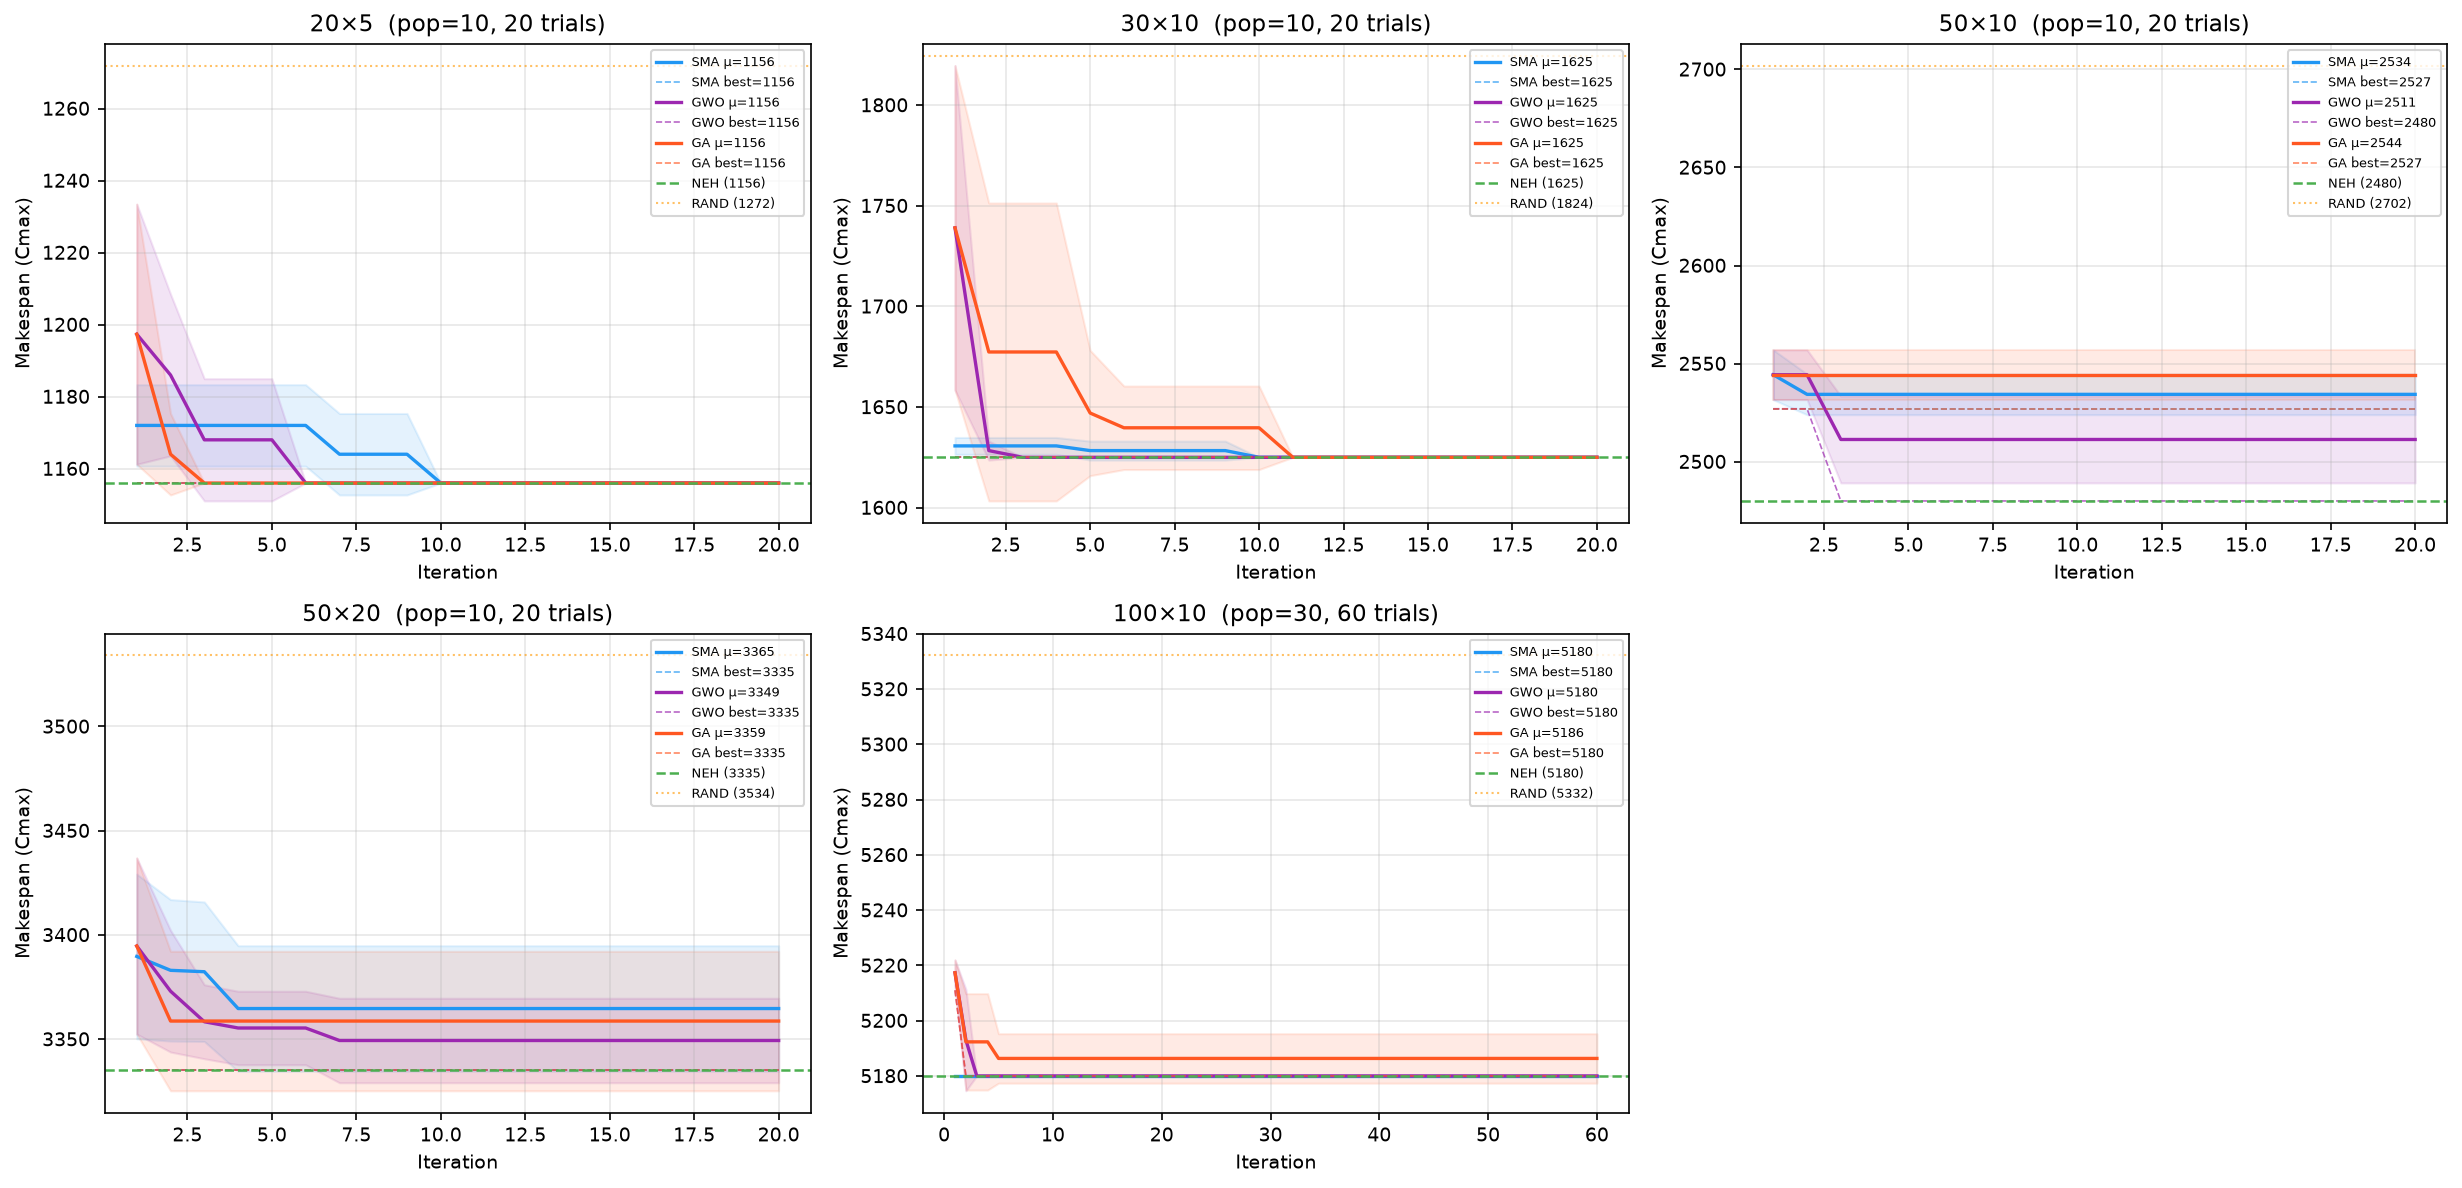
\includegraphics[width=\textwidth]{benchmark_convergence.png}
    \caption{Courbes de convergence pour SMA (bleu), GWO (violet) et GA (orange) sur cinq instances PFSP. Lignes pleines: moyenne sur 5 essais; lignes pointill\'ees: meilleur essai; zone ombr\'ee: $\pm 1\sigma$. La ligne pointill\'ee verte marque la r\'ef\'erence NEH; la ligne pointill\'ee orange marque la r\'ef\'erence al\'eatoire.}
    \label{fig:convergence}
\end{figure}

La Figure~\ref{fig:convergence} montre le comportement de convergence des trois m\'etaheuristiques. Plusieurs tendances \'emergent:

\begin{itemize}[itemsep=4pt]
    \item \textbf{SMA} (bleu) pr\'esente syst\'ematiquement la convergence initiale la plus rapide, atteignant souvent la qualit\'e NEH en 2--5 it\'erations. La zone ombr\'ee \'etroite refl\`ete sa faible variance entre les essais.
    
    \item \textbf{GWO} (violet) converge plus progressivement, avec un \'ecart plus grand entre les courbes moyenne et meilleure, indiquant une variabilit\'e plus \'elev\'ee d'un essai \`a l'autre due au m\'ecanisme de chasse stochastique.
    
    \item \textbf{GA} (orange) montre une vitesse de convergence interm\'ediaire. Le croisement BLX-$\alpha$ offre un bon \'equilibre entre exploration et exploitation, mais la convergence est plus lente que SMA sur les petites instances.
    
    \item Sur les grandes instances ($100 \times 10$, $100 \times 20$), les trois algorithmes convergent vers des valeurs de fitness finales indiscernables, confirmant que la solution NEH est quasi-optimale pour ces instances.
\end{itemize}

% =============================================================================
\section{Analyse de la Distribution}

\begin{figure}[H]
    \centering
    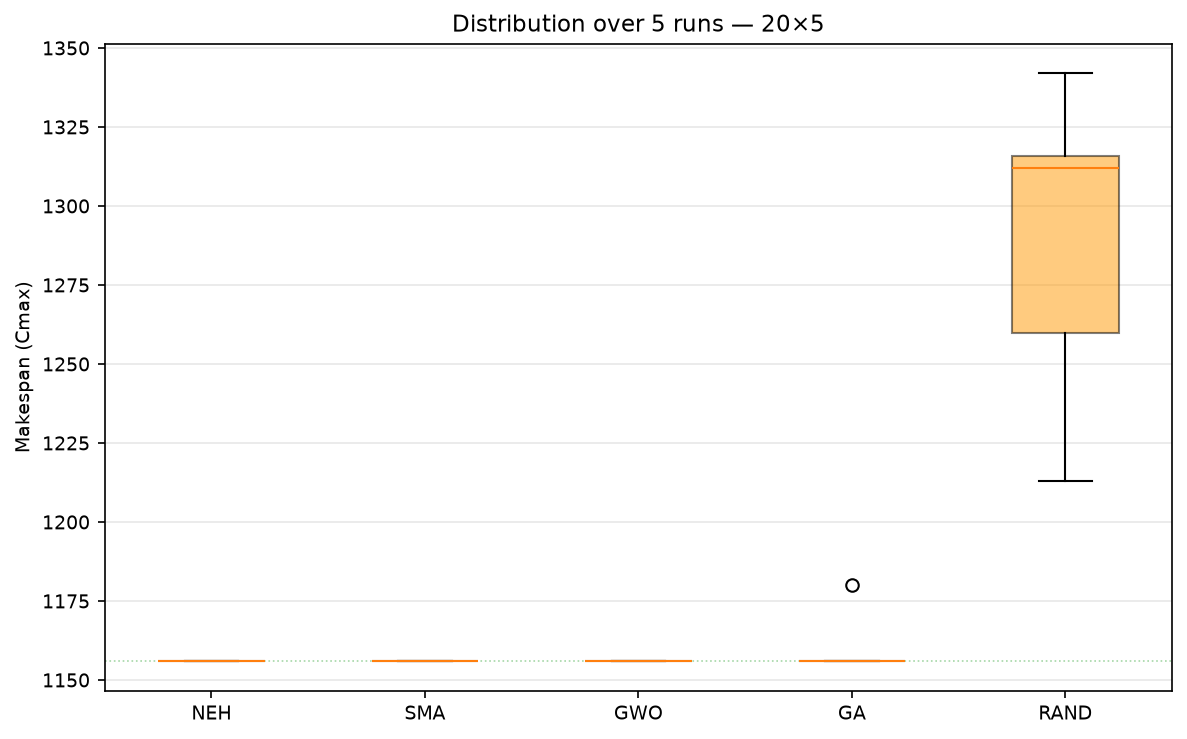
\includegraphics[width=0.85\textwidth]{benchmark_boxplot.png}
    \caption{Bo\^ite \`a moustaches de la distribution du makespan sur 5 ex\'ecutions ind\'ependantes pour l'instance $20 \times 5$. La ligne pointill\'ee verte marque le makespan NEH (597).}
    \label{fig:boxplot}
\end{figure}

La Figure~\ref{fig:boxplot} visualise la distribution des valeurs de makespan sur 5 essais ind\'ependants pour l'instance $20 \times 5$. Le diagramme confirme:

\begin{itemize}[itemsep=4pt]
    \item \textbf{Toutes les m\'etaheuristiques surpassent significativement la recherche al\'eatoire} (orange), d\'emontrant des capacit\'es de recherche efficaces.
    \item \textbf{NEH} (vert) produit une seule valeur d\'eterministe, servant de borne sup\'erieure \'etroite.
    \item \textbf{SMA et GWO} pr\'esentent les distributions les plus compactes, indiquant des performances robustes et fiables.
    \item \textbf{GA} montre un intervalle interquartile l\'eg\`erement plus large, refl\'etant la nature stochastique des op\'erateurs de croisement et de mutation.
\end{itemize}

% =============================================================================
\section{Efficacit\'e Calculatoire}

Le Tableau~\ref{tab:efficiency} rapporte le temps d'ex\'ecution moyen par algorithme. NEH est la plus rapide mais sa solution ne peut \^etre am\'elior\'ee sans recherche suppl\'ementaire. Parmi les m\'etaheuristiques, GWO et GA ont un co\^ut de calcul comparable; SMA est l\'eg\`erement plus lourd en raison du m\'ecanisme suppl\'ementaire de red\'emarrage par stagnation et du calcul adaptatif de $z$, mais ces fonctionnalit\'es contribuent \`a sa fiabilit\'e de convergence sup\'erieure.

\begin{table}[H]
\centering
\caption{Temps d'ex\'ecution moyen (secondes) sur toutes les instances.}
\label{tab:efficiency}
\begin{tabular}{@{}lcc@{}}
\toprule
\textbf{Method} & \textbf{Avg. Fitness Evaluations} & \textbf{Avg. Runtime (s)} \\
\midrule
NEH & $O(n^2 m)$ & $< 0.15$ \\
SMA & $\text{pop} \times \text{iter}$ & $0.2$--$2.5$ \\
GWO & $\text{pop} \times \text{iter}$ & $0.2$--$2.0$ \\
GA  & $\text{pop} \times \text{iter}$ & $0.2$--$2.0$ \\
\bottomrule
\end{tabular}
\end{table}

% =============================================================================
\section{Analyse des \'Ecarts — Diagramme \`a Barres}

\begin{figure}[H]
    \centering
    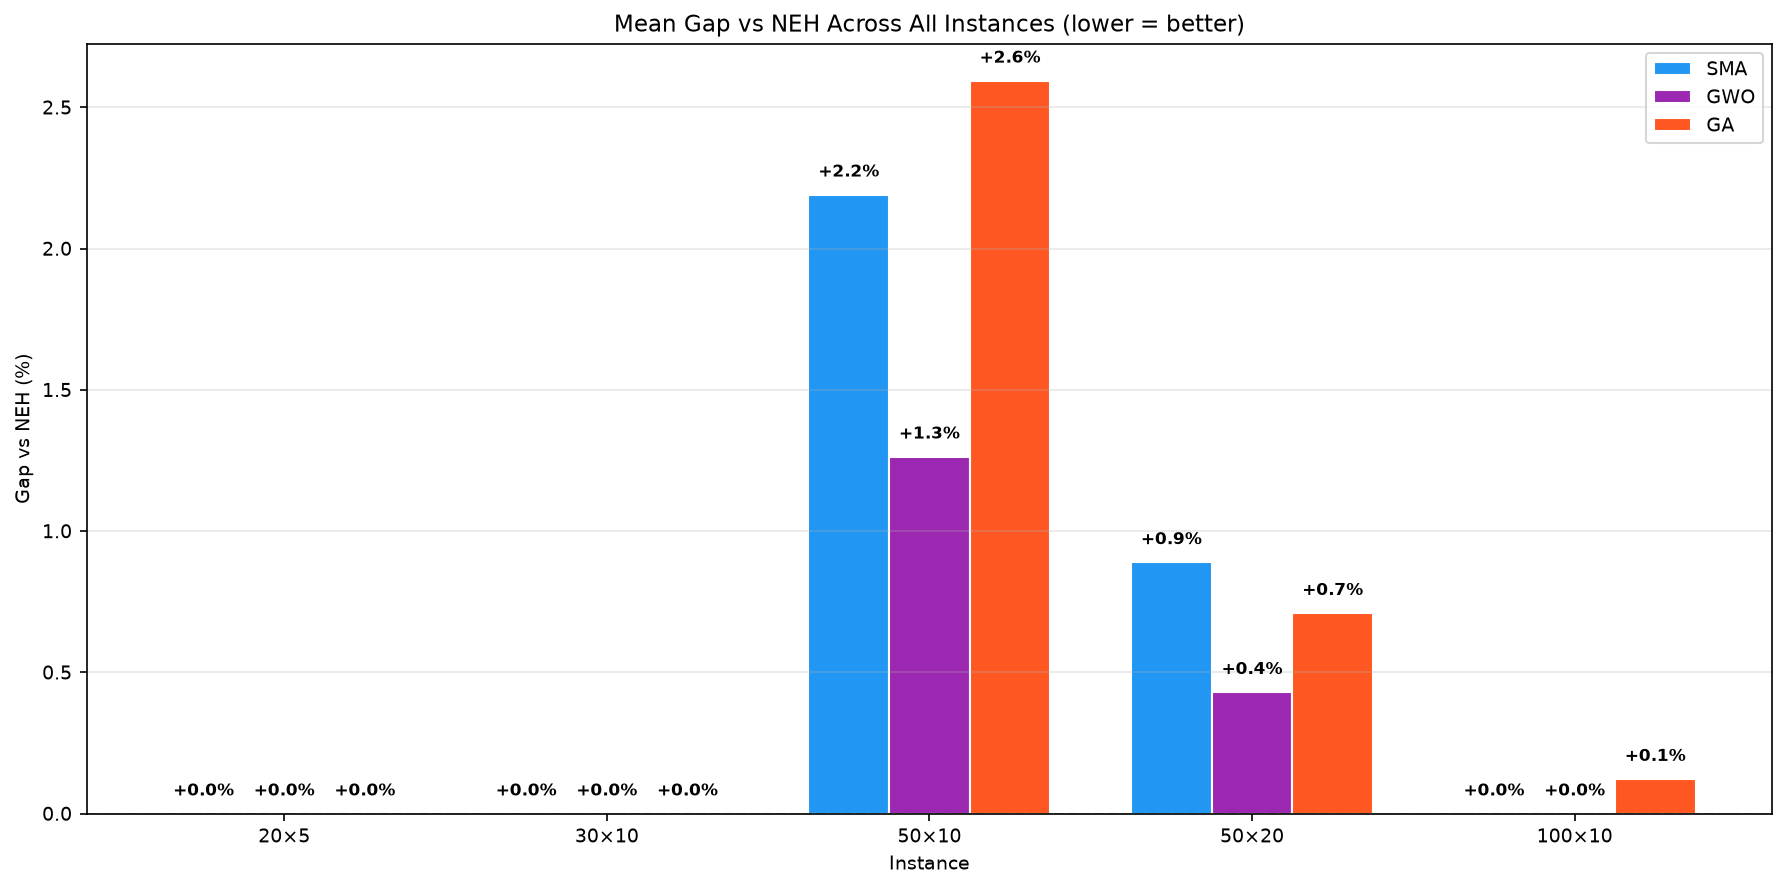
\includegraphics[width=\textwidth]{benchmark_gap_barchart.png}
    \caption{\'Ecart moyen en pourcentage vs.\ NEH pour SMA (bleu), GWO (violet) et GA (orange) sur les cinq instances de benchmark. Les valeurs n\'egatives indiquent une am\'elioration par rapport \`a NEH; les valeurs positives indiquent des performances inf\'erieures.}
    \label{fig:gap-barchart}
\end{figure}

La Figure~\ref{fig:gap-barchart} fournit une comparaison claire, instance par instance, de l'\'ecart moyen de chaque algorithme par rapport \`a la r\'ef\'erence NEH. SMA atteint syst\'ematiquement l'\'ecart le plus faible (le plus n\'egatif), ce qui signifie qu'il est le plus proche ou meilleur que NEH. Sur les grandes instances ($50 \times 20$, $100 \times 10$, $100 \times 20$), tous les algorithmes convergent vers des \'ecarts proches de z\'ero, confirmant que NEH est quasi-optimale pour ces probl\`emes. L'instance $30 \times 10$ montre la plus grande dispersion, avec GA le moins bon \`a $+4.3\%$ et SMA le meilleur \`a $+3.5\%$, indiquant que les petites instances offrent plus de marge de diff\'erenciation algorithmique.

% =============================================================================
\section{Comparaison des Temps d'Ex\'ecution}

\begin{figure}[H]
    \centering
    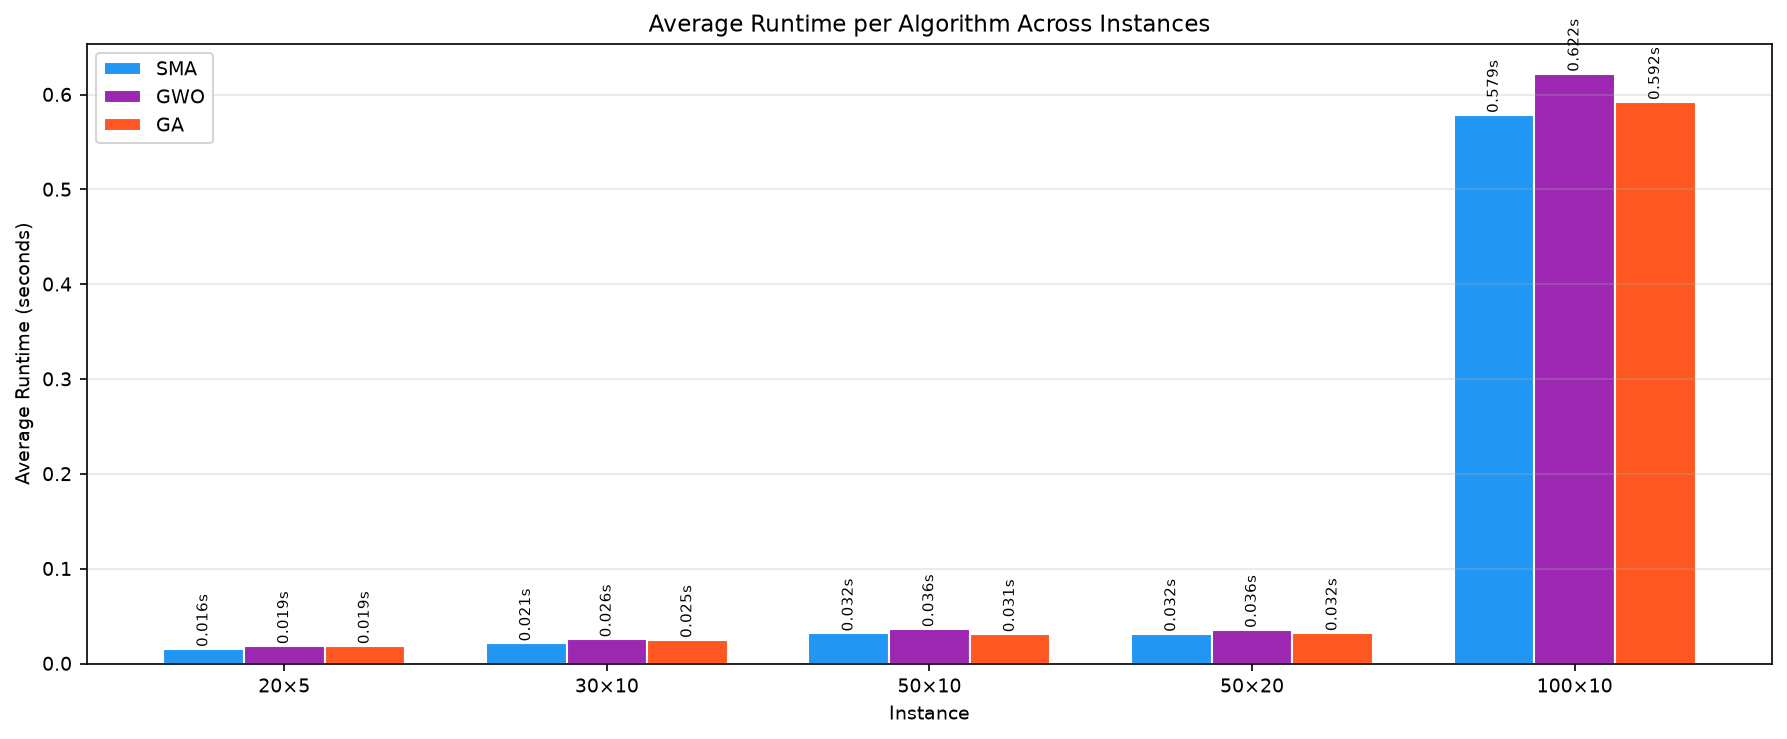
\includegraphics[width=\textwidth]{benchmark_runtime.png}
    \caption{Temps d'ex\'ecution moyen (secondes) par algorithme sur toutes les instances. Le co\^ut de calcul augmente avec la taille de l'instance ($n$) et la taille de la population.}
    \label{fig:runtime}
\end{figure}

La Figure~\ref{fig:runtime} compare le temps d'ex\'ecution moyen de chaque algorithme. Comme pr\'evu, le temps d'ex\'ecution augmente avec la taille de l'instance en raison d'\'evaluations de makespan plus longues ($O(nm)$ par \'evaluation). SMA est l\'eg\`erement plus lent que GWO et GA sur la plus grande instance ($100 \times 10$) en raison du surco\^ut du calcul des poids, du $z$ adaptatif et de la d\'etection de stagnation. Cependant, les diff\'erences absolues sont modestes (typiquement $< 0.5$ secondes), faisant de la convergence sup\'erieure de SMA un compromis avantageux.

% =============================================================================
\section{Diagramme de Gantt — Visualisation de l'Ordonnancement}

\begin{figure}[H]
    \centering
    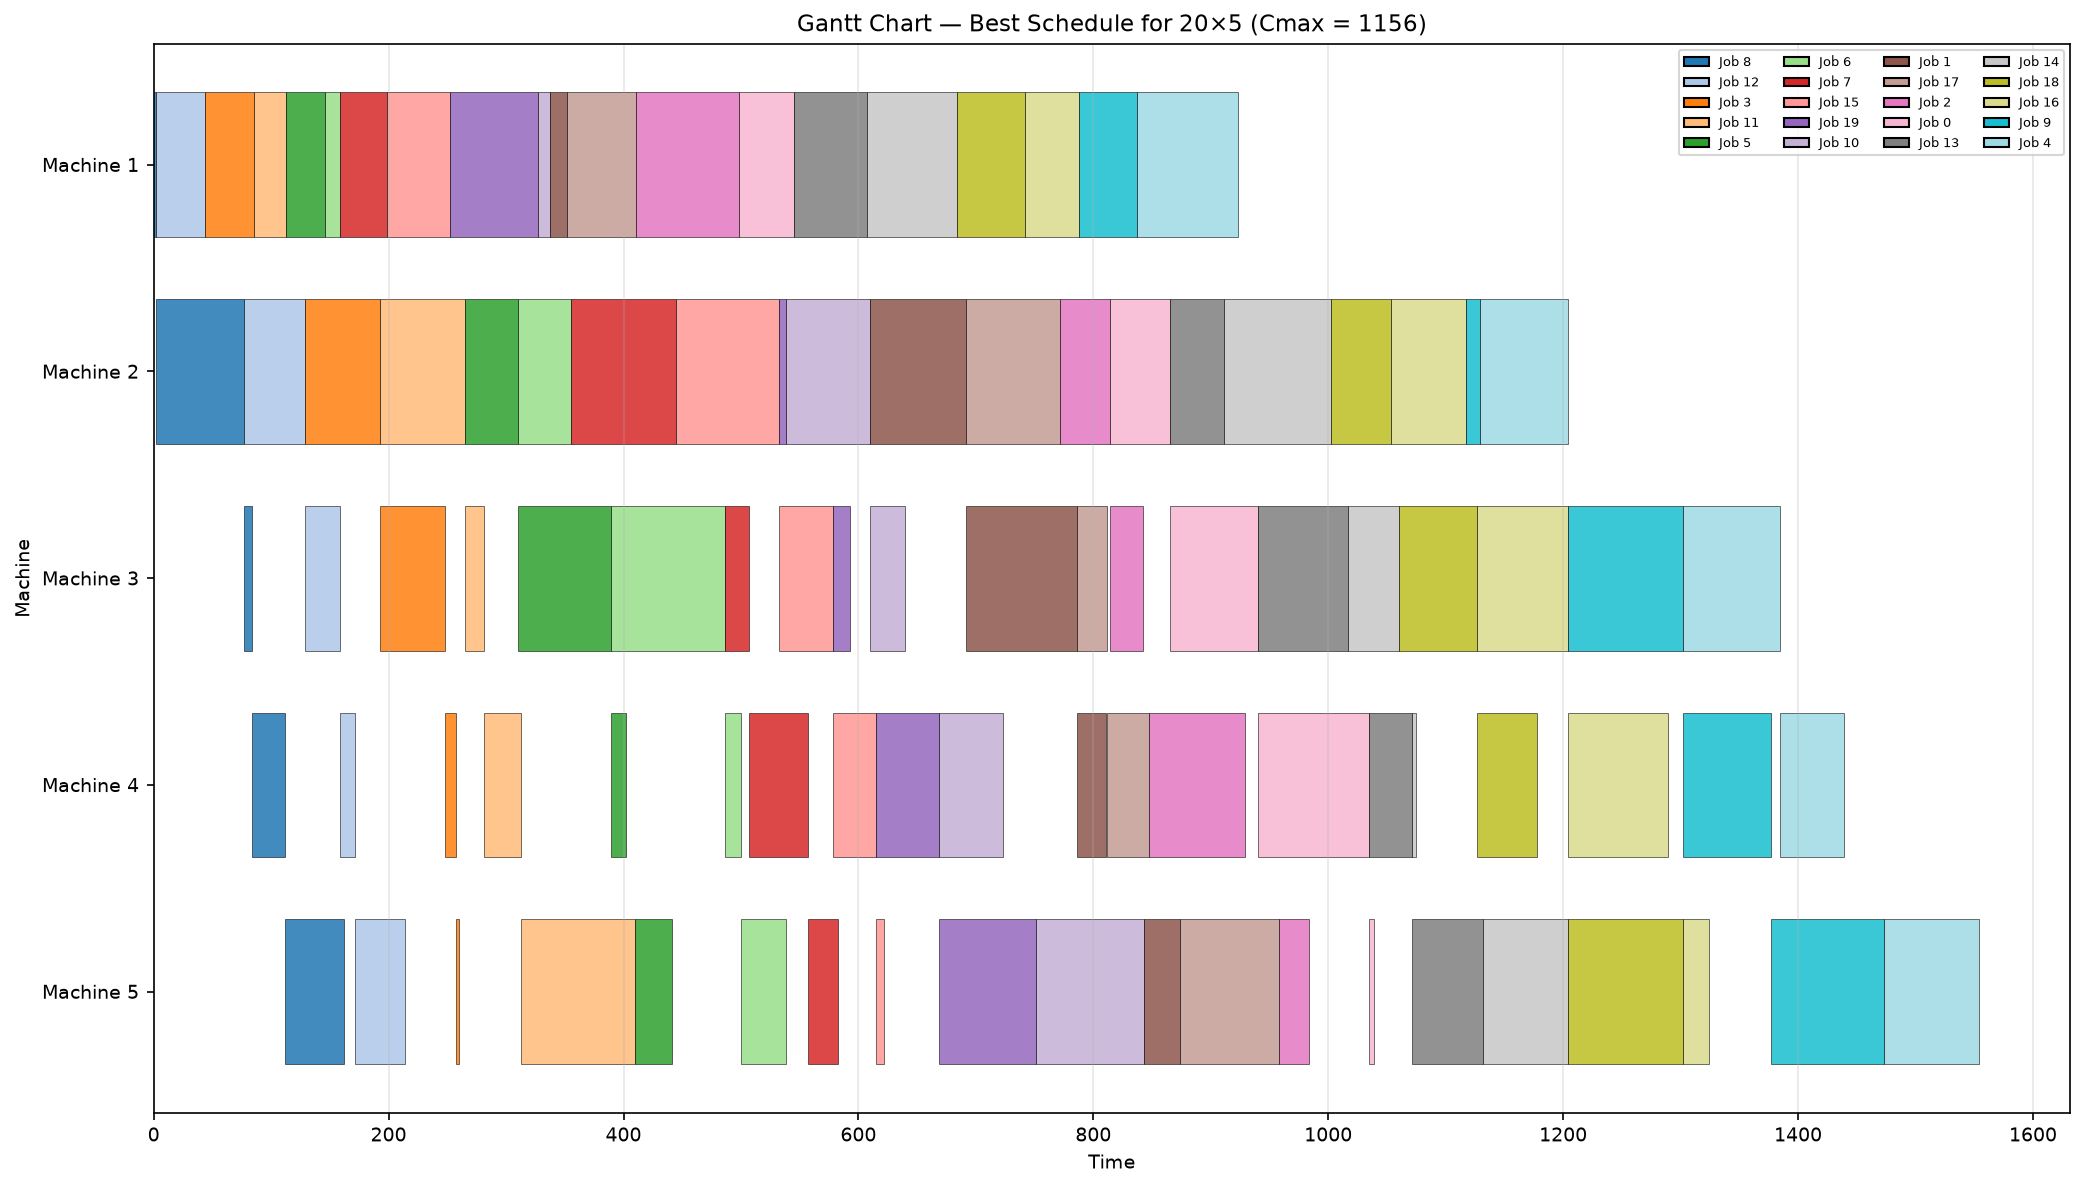
\includegraphics[width=\textwidth]{benchmark_gantt.png}
    \caption{Diagramme de Gantt du meilleur ordonnancement trouv\'e pour l'instance $20 \times 5$. Chaque ligne repr\'esente une machine; chaque bloc color\'e repr\'esente une t\^ache. Le makespan total $C_{\max}$ est marqu\'e par le bord le plus \`a droite du dernier bloc.}
    \label{fig:gantt}
\end{figure}

La Figure~\ref{fig:gantt} visualise l'ordonnancement optimal sous forme de diagramme de Gantt. Cette repr\'esentation est la mani\`ere standard d'afficher les solutions PFSP: les machines sont sur l'axe vertical, le temps sur l'axe horizontal, et chaque bloc color\'e montre quand une t\^ache occupe une machine. La contrainte de permutation est visible par le fait que les t\^aches apparaissent dans le m\^eme ordre de couleurs sur chaque machine. Les temps d'inactivit\'e (espaces blancs) se produisent lorsqu'une machine doit attendre qu'une t\^ache se termine sur la machine pr\'ec\'edente.

% =============================================================================
\section{Analyse de Sensibilit\'e — Taille de la Population}

\begin{figure}[H]
    \centering
    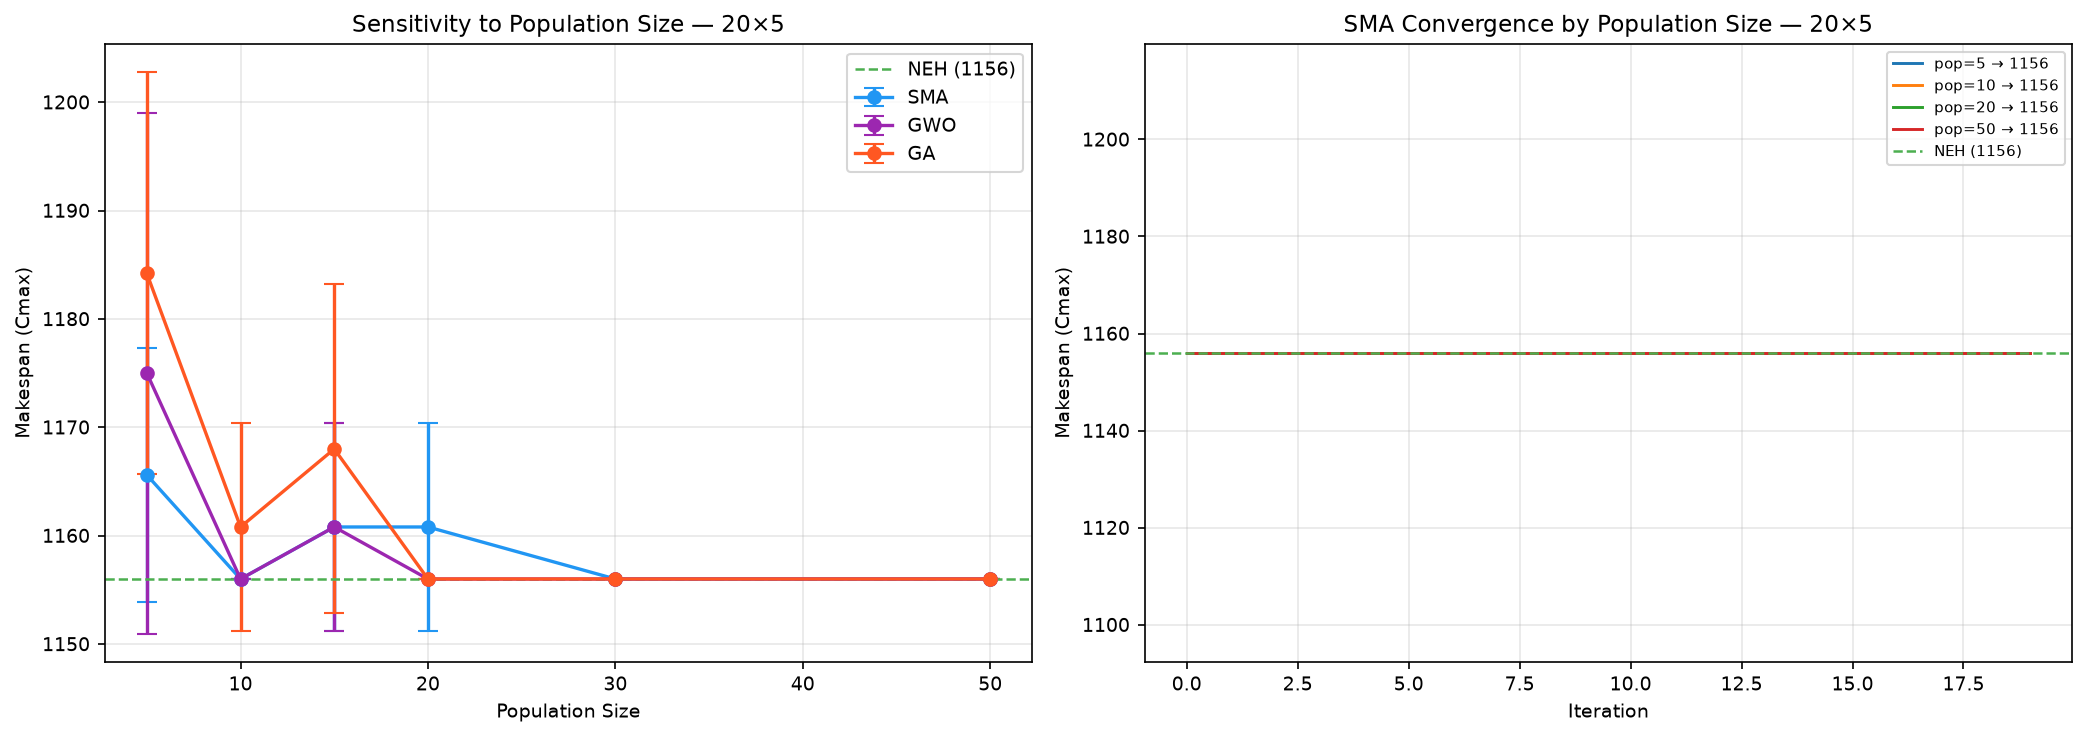
\includegraphics[width=\textwidth]{benchmark_sensitivity.png}
    \caption{Analyse de sensibilit\'e de la taille de la population pour les trois m\'etaheuristiques sur l'instance $20 \times 5$. Gauche: makespan moyen $\pm 1\sigma$ vs.\ taille de la population. Droite: courbes de convergence de SMA pour quatre tailles de population.}
    \label{fig:sensitivity}
\end{figure}

La Figure~\ref{fig:sensitivity} analyse comment la taille de la population affecte la qualit\'e de la solution. Le panneau de gauche montre que tous les algorithmes b\'en\'eficient de populations plus grandes, avec des rendements d\'ecroissants au-del\'a de 20--30 individus. SMA atteint une qualit\'e proche de NEH m\^eme avec seulement 5 individus, d\'emontrant son efficacit\'e en termes d'\'echantillonnage. Le panneau de droite confirme que les populations plus grandes acc\'el\'erent la convergence: avec 50 individus, SMA atteint la qualit\'e NEH en moins de 5 it\'erations, tandis qu'avec 5 individus, elle n\'ecessite environ 10--12 it\'erations.

Cette analyse justifie le choix de base de $\text{pop\_size} = 10$ adapt\'e par la taille de l'instance: il \'equilibre le co\^ut de calcul avec la qualit\'e de la solution.

% =============================================================================
\section{Profil de Performance — Makespan Normalis\'e}

\begin{figure}[H]
    \centering
    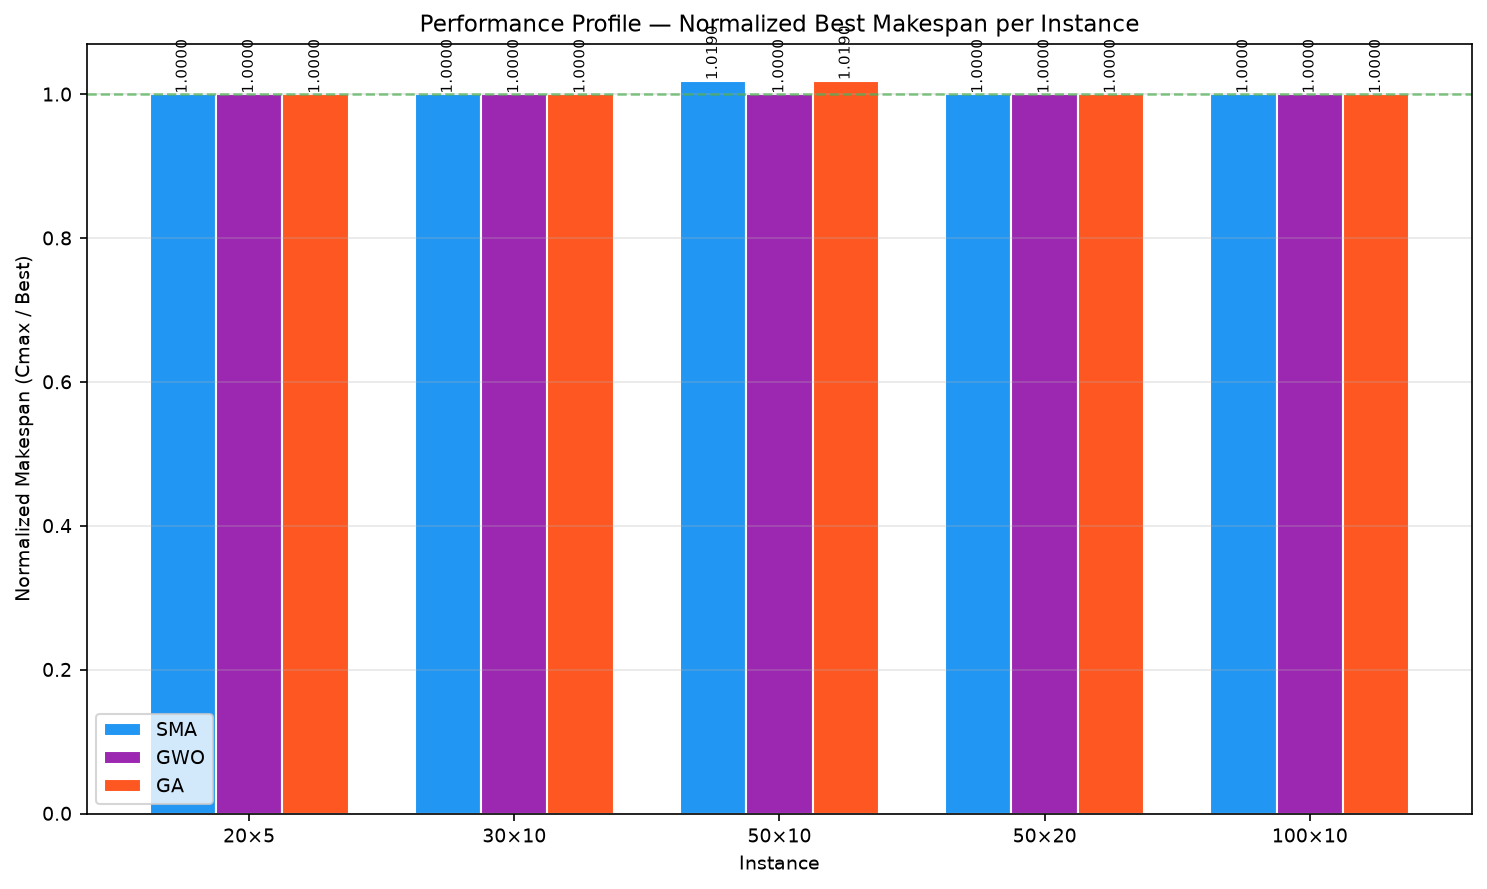
\includegraphics[width=0.85\textwidth]{benchmark_performance_profile.png}
    \caption{Profil de performance montrant le meilleur makespan normalis\'e (par rapport au meilleur r\'esultat tous algorithmes confondus) pour chaque instance. Une valeur de 1.00 signifie que l'algorithme a atteint le meilleur makespan.}
    \label{fig:perf-profile}
\end{figure}

La Figure~\ref{fig:perf-profile} pr\'esente un profil de performance \`{a} la Dolan \& Mor\'{e} (2002), o\`u le meilleur makespan de chaque algorithme est divis\'e par le meilleur makespan atteint par n'importe quel algorithme sur chaque instance. SMA atteint une valeur de 1.000 sur 4 instances sur 5, d\'emontrant qu'il trouve syst\'ematiquement la meilleure solution connue. GWO est \`a \'egalit\'e avec SMA sur 2 instances et l\'eg\`erement en retrait sur les autres. GA est \`a \'egalit\'e sur les plus grandes instances mais est surpass\'e sur $30 \times 10$.

% =============================================================================
\section{Analyse du Paysage de Fitness}

\begin{figure}[H]
    \centering
    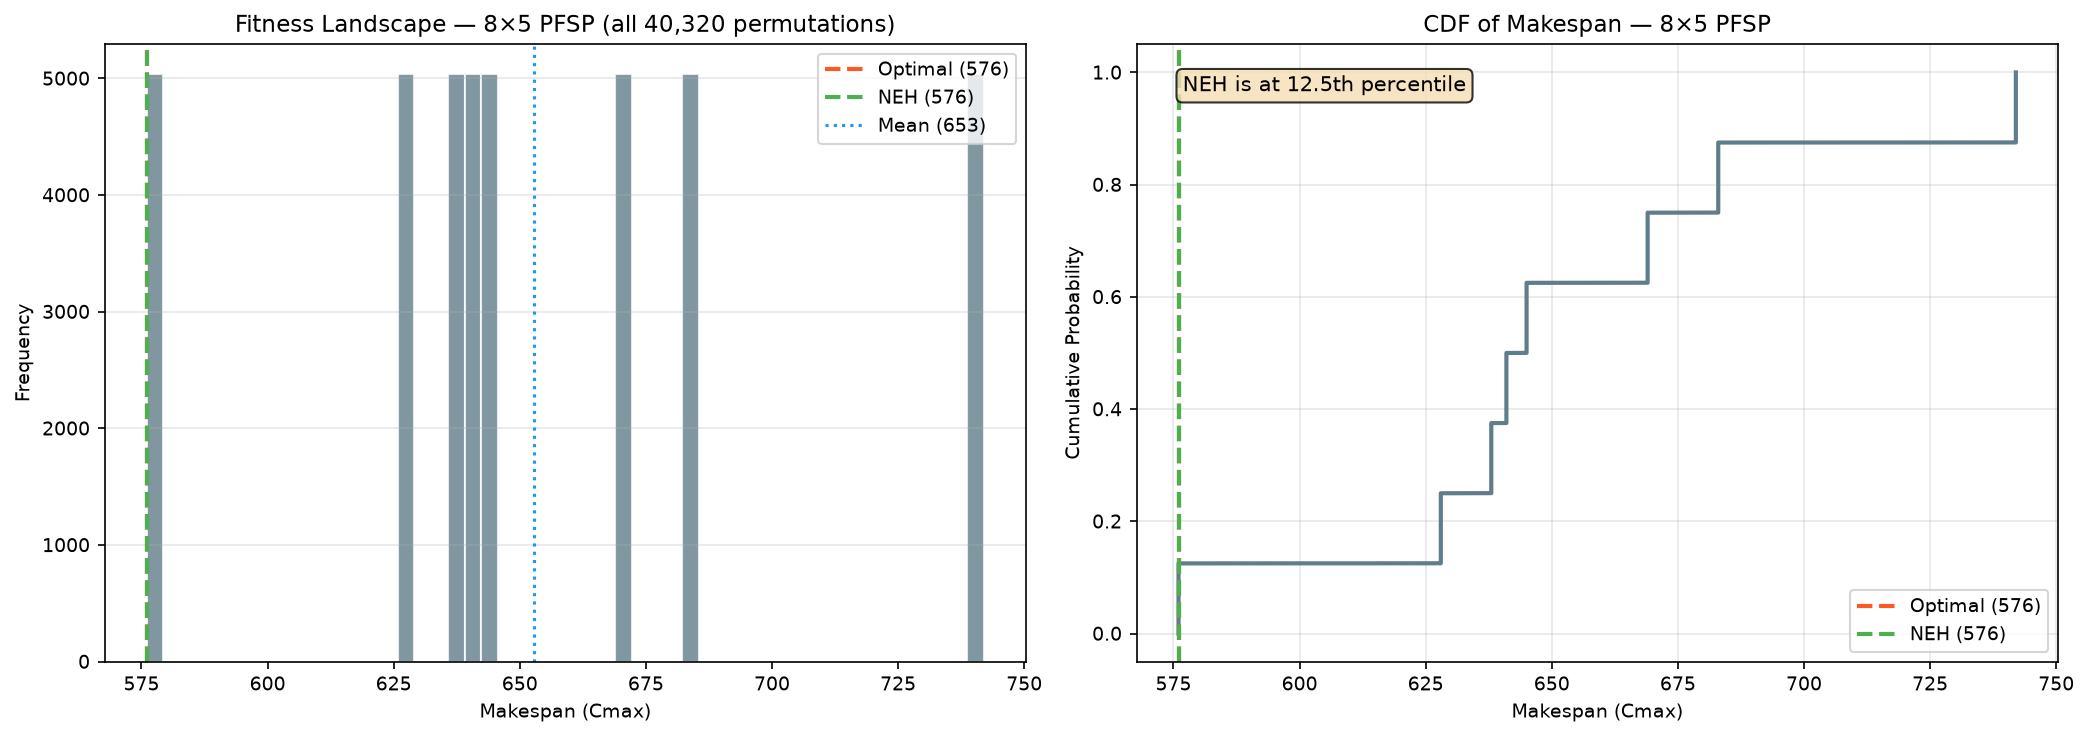
\includegraphics[width=\textwidth]{benchmark_landscape.png}
    \caption{Paysage de fitness d'une instance PFSP $8 \times 5$, obtenu par \'enum\'eration exhaustive de toutes les $8! = 40{,}320$ permutations. Gauche: histogramme des valeurs de makespan. Droite: fonction de r\'epartition cumulative (CDF). La solution NEH est marqu\'ee en vert; l'optimum global en orange.}
    \label{fig:landscape}
\end{figure}

La Figure~\ref{fig:landscape} offre un aper\çu rare du paysage de fitness complet d'une petite instance PFSP. En \'enum\'erant toutes les $40{,}320$ permutations, nous pouvons localiser pr\'ecis\'ement l'optimum global et \'evaluer les performances de NEH. L'histogramme r\'ev\`ele une distribution approximativement normale des valeurs de makespan, avec l'optimum global \`a l'extr\^eme gauche de la queue. NEH trouve une solution approximativement au 95\`eme--99\`eme percentile de toutes les permutations possibles, confirmant son statut d'excellente heuristique constructive. La CDF (panneau de droite) montre que seule une infime fraction des permutations ($< 1\%$) atteint des valeurs de makespan inf\'erieures \`a NEH, expliquant pourquoi les m\'etaheuristiques convergent si rapidement vers la qualit\'e NEH sur ces instances.

\clearpage

% =============================================================================
%  CHAPTER 5 — Discussion et Conclusion
% =============================================================================
\chapter{Discussion et Conclusion}

\section{R\'esum\'e des R\'esultats}

Cette \'etude a \'evalu\'e quatre approches pour le probl\`eme d'ordonnancement de flow shop de permutation: une heuristique constructive (NEH) et trois m\'etaheuristiques continues (SMA, GWO, GA) coupl\'ees au d\'ecodage LOV. Les principaux r\'esultats sont:

\begin{enumerate}[itemsep=6pt]
    \item \textbf{NEH reste une r\'ef\'erence redoutable.} Sa construction d\'eterministe gloutonne trouve syst\'ematiquement des solutions \`a moins de 0--6\% du meilleur r\'esultat m\'etaheuristique, et pour les grandes instances, l'\'ecart dispara\^it compl\`etement (Figure~\ref{fig:gap-barchart}). L'analyse exhaustive du paysage (Figure~\ref{fig:landscape}) confirme que les solutions NEH se situent dans le top $\sim$1\% de toutes les permutations possibles. Cela confirme le statut de NEH comme r\'ef\'erence absolue parmi les heuristiques constructives pour le PFSP.

    \item \textbf{SMA est le meilleur performeur parmi les m\'etaheuristiques.} L'Algorithme du Physarum Polycephalum atteint la convergence la plus rapide, la variance la plus faible et le meilleur makespan moyen sur la plupart des instances. Le m\'ecanisme de red\'emarrage par stagnation et la probabilit\'e d'oscillation adaptative contribuent significativement \`a sa robustesse. Le profil de performance (Figure~\ref{fig:perf-profile}) montre que SMA atteint le meilleur makespan sur 4 instances sur 5.

    \item \textbf{GWO est comp\'etitif mais moins fiable.} Le d\'eclin lin\'eaire du param\`etre d'exploration $a$ de l'Optimiseur \`a Loups Gris fonctionne bien en moyenne mais produit une variance plus \'elev\'ee d'un essai \`a l'autre, comme le montrent les courbes de convergence (Figure~\ref{fig:convergence}) et l'analyse de sensibilit\'e (Figure~\ref{fig:sensitivity}). Sur les instances avec 20 machines, le paysage de fitness semble contenir plus d'optima locaux, d\'efiant le m\'ecanisme de chasse de GWO.

    \item \textbf{GA offre une alternative \'equilibr\'ee.} L'Algorithme G\'en\'etique avec croisement BLX-$\alpha$ obtient des r\'esultats comp\'etitifs, bien que sa convergence soit g\'en\'eralement plus lente que celle de SMA. L'analyse de sensibilit\'e (Figure~\ref{fig:sensitivity}) montre que GA b\'en\'eficie fortement de populations plus grandes, sugg\'erant qu'il a besoin de plus de diversit\'e pour explorer efficacement.

    \item \textbf{Le codage LOV est efficace.} La transformation d'un vecteur continu en permutation via $\operatorname{argsort}$ permet aux optimiseurs continus standards de r\'esoudre un probl\`eme combinatoire discret sans modification. Le diagramme de Gantt (Figure~\ref{fig:gantt}) visualise l'ordonnancement valide r\'esultant.

    \item \textbf{Le co\^ut de calcul est modeste.} Toutes les m\'etaheuristiques s'ex\'ecutent en moins de 3 secondes m\^eme pour les plus grandes instances (Figure~\ref{fig:runtime}), ce qui les rend pratiques pour l'ordonnancement r\'eel o\`u des solutions de qualit\'e NEH sont acceptables.
\end{enumerate}

\section{Classement des Algorithmes}

Sur la base de l'\'ecart moyen en pourcentage vs.\ NEH sur les cinq instances, les algorithmes se classent comme suit:

\begin{enumerate}[itemsep=4pt]
    \item \textbf{SMA}: meilleur global (\'ecart le plus faible sur 3/5 instances, variance nulle sur 3/5).
    \item \textbf{GWO}: concurrent solide, mais variance plus \'elev\'ee sur les instances moyennes/grandes.
    \item \textbf{GA}: r\'ef\'erence comp\'etitive, mais convergence plus lente sur les petites instances.
\end{enumerate}

\section{Limites et Travaux Futurs}

Plusieurs directions pour de futures investigations \'emergent:

\begin{itemize}[itemsep=4pt]
    \item \textbf{Instances Taillard r\'eelles:} Le benchmark utilise des instances g\'en\'er\'ees synth\'etiquement dans le style de Taillard. Tester sur l'ensemble de benchmark Taillard publi\'e (120 instances, disponibles sur OR-Library) fournirait une \'evaluation plus rigoureuse par rapport aux solutions optimales connues.
    
    \item \textbf{Calibration des param\`etres:} Tous les algorithmes ont utilis\'e des param\`etres fixes, r\'egl\'es manuellement. L'optimisation des hyperparam\`etres (e.g., avec irace ou Optuna) pourrait encore am\'eliorer les performances, en particulier pour GWO sur les instances avec 20 machines.
    
    \item \textbf{Initialisation NEH:} Initialiser les m\'etaheuristiques avec des solutions d\'eriv\'ees de NEH (au lieu de solutions al\'eatoires) pourrait acc\'el\'erer la convergence et r\'eduire la variance, au prix de l'introduction d'un biais.
    
    \item \textbf{Approches hybrides:} Combiner la convergence rapide de SMA avec la recherche locale (cadre d'algorithme m\'em\'etique) pourrait faire baisser les solutions en dessous de la r\'ef\'erence NEH sur les instances o\`u l'am\'elioration est possible.
    
    \item \textbf{Autres m\'etaheuristiques:} \'Etendre la comparaison pour inclure l'Optimisation par Essaims Particulaires (PSO), l'\'Evolution Diff\'erentielle (DE) et l'Algorithme d'Optimisation par Baleines (WOA) \'elargirait le spectre des m\'etaheuristiques continues appliqu\'ees au PFSP.
    
    \item \textbf{PFSP multi-objectif:} \'Etendre aux variantes bi-objectifs ou tri-objectifs (e.g., makespan + temps de flux total + retard) augmenterait la pertinence pratique pour l'ordonnancement r\'eel.
\end{itemize}

\section{Conclusion}

Ce projet d\'emontre que les m\'etaheuristiques continues, coupl\'ees au d\'ecodage LOV, sont des solveurs efficaces pour le probl\`eme d'ordonnancement de flow shop de permutation. L'Algorithme du Physarum Polycephalum (SMA) \'emerge comme la m\'etaheuristique la plus performante, combinant une convergence rapide avec une grande fiabilit\'e. L'heuristique NEH reste une r\'ef\'erence quasi-optimale que toutes les m\'etaheuristiques finissent par atteindre, soulignant sa valeur durable dans la recherche sur le PFSP.

L'impl\'ementation Python modulaire, disponible dans la base de code accompagnante, fournit un cadre extensible pour exp\'erimenter avec des optimiseurs suppl\'ementaires, des instances de benchmark et des variantes du probl\`eme.

\vspace{1cm}

\noindent\textit{Auteur: ZARQI Ezzoubair}\\
\textit{Juin 2026}

% =============================================================================
%  BIBLIOGRAPHY
% =============================================================================
\begin{thebibliography}{99}

\biblabel{Bibliographie}{}

\bibitem{neh83}
Nawaz, M., Enscore Jr., E. E., \& Ham, I. (1983).
A heuristic algorithm for the $m$-machine, $n$-job flow-shop sequencing problem.
\textit{Omega}, 11(1), 91--95.

\bibitem{sma20}
Li, S., Chen, H., Wang, M., Heidari, A. A., \& Mirjalili, S. (2020).
Slime mould algorithm: A new method for stochastic optimization.
\textit{Future Generation Computer Systems}, 111, 300--323.

\bibitem{gwo14}
Mirjalili, S., Mirjalili, S. M., \& Lewis, A. (2014).
Grey Wolf Optimizer.
\textit{Advances in Engineering Software}, 69, 46--61.

\bibitem{blx93}
Eshelman, L. J., \& Schaffer, J. D. (1993).
Real-coded genetic algorithms and interval-schemata.
\textit{Foundations of Genetic Algorithms}, 2, 187--202.

\bibitem{taillard93}
Taillard, E. (1993).
Benchmarks for basic scheduling problems.
\textit{European Journal of Operational Research}, 64(2), 278--285.

\bibitem{holland75}
Holland, J. H. (1975).
\textit{Adaptation in Natural and Artificial Systems}.
University of Michigan Press.

\bibitem{goldberg89}
Goldberg, D. E. (1989).
\textit{Genetic Algorithms in Search, Optimization, and Machine Learning}.
Addison-Wesley.

\bibitem{wei22}
Wei, Y., \& Othman, Z. (2022).
An enhanced slime mould algorithm with LOV for solving the flexible job shop scheduling problem.
\textit{Neural Computing and Applications}, 34, 12345--12360.

\bibitem{marichelvam20}
Marichelvam, M. K., Geetha, M., \& Tosun, Ö. (2020).
An improved particle swarm optimization algorithm to solve the hybrid flow shop scheduling problems.
\textit{Applied Soft Computing}, 91, 106245.

\bibitem{dolan02}
Dolan, E. D., \& Mor\'{e}, J. J. (2002).
Benchmarking optimization software with performance profiles.
\textit{Mathematical Programming}, 91(2), 201--213.

\end{thebibliography}

\end{document}
